%
% The 2-D CCD Data Reduction Cookbook
%
% Copyright 2001 Starlink, CCLRC.
%
% A.C. Davenhall (Edinburgh), 16/8/01.
%

\documentclass[twoside,11pt]{article}

% ? Specify used packages
\usepackage{graphicx}        %  Use this one for final production.
% \usepackage[draft]{graphicx} %  Use this one for drafting.
% ? End of specify used packages

\pagestyle{myheadings}

% -----------------------------------------------------------------------------
% ? Document identification
% Fixed part
\newcommand{\stardoccategory}  {Starlink Cookbook}
\newcommand{\stardocinitials}  {SC}
\newcommand{\stardocsource}    {sc\stardocnumber}
\newcommand{\stardoccopyright} {Copyright \copyright\ 2001 Council for the
Central Laboratory of the Research Councils}

% Variable part - replace [xxx] as appropriate.
\newcommand{\stardocnumber}    {5.3}
\newcommand{\stardocauthors}   {A.C.~Davenhall, G.J.~Privett \& M.B.~Taylor}
\newcommand{\stardocdate}      {16th August 2001}
\newcommand{\stardoctitle}     {The 2-D CCD Data Reduction Cookbook}
\newcommand{\stardocabstract}
{This cookbook presents simple recipes and scripts for reducing direct
images acquired with optical CCD detectors.  Using these recipes and
scripts you can correct un-processed images obtained from CCDs for
various instrumental effects to retrieve an accurate picture of the
field of sky observed.  The recipes and scripts use standard software
available at all Starlink sites.

The topics covered include: creating and applying bias and flat-field
corrections, registering frames and creating a stack or mosaic of
registered frames.  Related auxiliary tasks, such as converting between
different data formats, displaying images and calculating image statistics
are also presented.

In addition to the recipes and scripts, sufficient background material
is presented to explain the procedures and techniques used.  The
treatment is deliberately practical rather than theoretical, in keeping
with the aim of providing advice on the actual reduction of observations.
Additional material outlines some of the differences between using
conventional optical CCDs and the similar arrays used to observe at
infrared wavelengths.

\latex{\vspace{5mm}}

\begin{center}
{\bf Who Should Read this Cookbook?}
\end{center}

This cookbook is aimed firmly at people who are new to reducing CCD
observations.  Typical readers might have a set of CCD observations to
reduce (perhaps for the first time) or be planning to observe with a
CCD camera.  No prior knowledge of CCD data reduction is assumed.}
% ? End of document identification
% -----------------------------------------------------------------------------

% +
%  Name:
%     sc.tex
%
%  Purpose:
%     Template for Starlink Cookbook (SC) documents.
%     Refer to SUN/199
%
%  Authors:
%     AJC: A.J.Chipperfield (Starlink, RAL)
%     BLY: M.J.Bly (Starlink, RAL)
%
%  History:
%     16-JUN-1997 (BLY):
%        Original, based on SUN/SG templates.
%     {Add further history here}
%
% -

\newcommand{\stardocname}{\stardocinitials /\stardocnumber}
\markboth{\stardocname}{\stardocname}
\setlength{\textwidth}{160mm}
\setlength{\textheight}{230mm}
\setlength{\topmargin}{-2mm}
\setlength{\oddsidemargin}{0mm}
\setlength{\evensidemargin}{0mm}
\setlength{\parindent}{0mm}
\setlength{\parskip}{\medskipamount}
\setlength{\unitlength}{1mm}

% -----------------------------------------------------------------------------
%  Hypertext definitions.
%  ======================
%  These are used by the LaTeX2HTML translator in conjunction with star2html.

%  Comment.sty: version 2.0, 19 June 1992
%  Selectively in/exclude pieces of text.
%
%  Author
%    Victor Eijkhout                                      <eijkhout@cs.utk.edu>
%    Department of Computer Science
%    University Tennessee at Knoxville
%    104 Ayres Hall
%    Knoxville, TN 37996
%    USA

%  Do not remove the %begin{latexonly} and %end{latexonly} lines (used by 
%  star2html to signify raw TeX that latex2html cannot process).
%begin{latexonly}
\makeatletter
\def\makeinnocent#1{\catcode`#1=12 }
\def\csarg#1#2{\expandafter#1\csname#2\endcsname}

\def\ThrowAwayComment#1{\begingroup
    \def\CurrentComment{#1}%
    \let\do\makeinnocent \dospecials
    \makeinnocent\^^L% and whatever other special cases
    \endlinechar`\^^M \catcode`\^^M=12 \xComment}
{\catcode`\^^M=12 \endlinechar=-1 %
 \gdef\xComment#1^^M{\def\test{#1}
      \csarg\ifx{PlainEnd\CurrentComment Test}\test
          \let\html@next\endgroup
      \else \csarg\ifx{LaLaEnd\CurrentComment Test}\test
            \edef\html@next{\endgroup\noexpand\end{\CurrentComment}}
      \else \let\html@next\xComment
      \fi \fi \html@next}
}
\makeatother

\def\includecomment
 #1{\expandafter\def\csname#1\endcsname{}%
    \expandafter\def\csname end#1\endcsname{}}
\def\excludecomment
 #1{\expandafter\def\csname#1\endcsname{\ThrowAwayComment{#1}}%
    {\escapechar=-1\relax
     \csarg\xdef{PlainEnd#1Test}{\string\\end#1}%
     \csarg\xdef{LaLaEnd#1Test}{\string\\end\string\{#1\string\}}%
    }}

%  Define environments that ignore their contents.
\excludecomment{comment}
\excludecomment{rawhtml}
\excludecomment{htmlonly}

%  Hypertext commands etc. This is a condensed version of the html.sty
%  file supplied with LaTeX2HTML by: Nikos Drakos <nikos@cbl.leeds.ac.uk> &
%  Jelle van Zeijl <jvzeijl@isou17.estec.esa.nl>. The LaTeX2HTML documentation
%  should be consulted about all commands (and the environments defined above)
%  except \xref and \xlabel which are Starlink specific.

\newcommand{\htmladdnormallinkfoot}[2]{#1\footnote{#2}}
\newcommand{\htmladdnormallink}[2]{#1}
\newcommand{\htmladdimg}[1]{}
\newenvironment{latexonly}{}{}
\newcommand{\hyperref}[4]{#2\ref{#4}#3}
\newcommand{\htmlref}[2]{#1}
\newcommand{\htmlimage}[1]{}
\newcommand{\htmladdtonavigation}[1]{}

% Define commands for HTML-only or LaTeX-only text.
\newcommand{\html}[1]{}
\newcommand{\latex}[1]{#1}

% Use latex2html 98.2.
\newcommand{\latexhtml}[2]{#1}

%  Starlink cross-references and labels.
\newcommand{\xref}[3]{#1}
\newcommand{\xlabel}[1]{}

%  LaTeX2HTML symbol.
\newcommand{\latextohtml}{{\bf LaTeX}{2}{\tt{HTML}}}

%  Define command to re-centre underscore for Latex and leave as normal
%  for HTML (severe problems with \_ in tabbing environments and \_\_
%  generally otherwise).
\newcommand{\setunderscore}{\renewcommand{\_}{{\tt\symbol{95}}}}
\latex{\setunderscore}

% -----------------------------------------------------------------------------
%  Debugging.
%  =========
%  Remove % from the following to debug links in the HTML version using Latex.

% \newcommand{\hotlink}[2]{\fbox{\begin{tabular}[t]{@{}c@{}}#1\\\hline{\footnotesize #2}\end{tabular}}}
% \renewcommand{\htmladdnormallinkfoot}[2]{\hotlink{#1}{#2}}
% \renewcommand{\htmladdnormallink}[2]{\hotlink{#1}{#2}}
% \renewcommand{\hyperref}[4]{\hotlink{#1}{\S\ref{#4}}}
% \renewcommand{\htmlref}[2]{\hotlink{#1}{\S\ref{#2}}}
% \renewcommand{\xref}[3]{\hotlink{#1}{#2 -- #3}}
%end{latexonly}
% -----------------------------------------------------------------------------
% ? Document-specific \newcommand or \newenvironment commands.
% ? End of document-specific commands
% -----------------------------------------------------------------------------
%  Title Page.
%  ===========
\renewcommand{\thepage}{\roman{page}}
\begin{document}
\thispagestyle{empty}

%  Latex document header.
%  ======================
\begin{latexonly}
   CCLRC / {\sc Rutherford Appleton Laboratory} \hfill {\bf \stardocname}\\
   {\large Particle Physics \& Astronomy Research Council}\\
   {\large Starlink Project\\}
   {\large \stardoccategory\ \stardocnumber}
   \begin{flushright}
   \stardocauthors\\
   \stardocdate
   \end{flushright}
   \vspace{-4mm}
   \rule{\textwidth}{0.5mm}
   \vspace{5mm}
   \begin{center}
   {\Huge\bf  \stardoctitle \\ [2.5ex]}
   \end{center}
   \vspace{5mm}

% ? Add picture here if required for the LaTeX version.
%   e.g. \includegraphics[scale=0.3]{filename.ps}
% ? End of picture

% ? Heading for abstract if used.
   \vspace{10mm}
   \begin{center}
      {\Large\bf Abstract}
   \end{center}
% ? End of heading for abstract.
\end{latexonly}

%  HTML documentation header.
%  ==========================
\begin{htmlonly}
   \xlabel{}
   \begin{rawhtml} <H1> \end{rawhtml}
      \stardoctitle
   \begin{rawhtml} </H1> \end{rawhtml}

% ? Add picture here if required for the hypertext version.
%   e.g. \includegraphics[scale=0.7]{filename.ps}
% ? End of picture

   \begin{rawhtml} <P> <I> \end{rawhtml}
   \stardoccategory\ \stardocnumber \\
   \stardocauthors \\
   \stardocdate
   \begin{rawhtml} </I> </P> <H3> \end{rawhtml}
      \htmladdnormallink{CCLRC}{http://www.cclrc.ac.uk} /
      \htmladdnormallink{Rutherford Appleton Laboratory}
                        {http://www.cclrc.ac.uk/ral} \\
      \htmladdnormallink{Particle Physics \& Astronomy Research Council}
                        {http://www.pparc.ac.uk} \\
   \begin{rawhtml} </H3> <H2> \end{rawhtml}
      \htmladdnormallink{Starlink Project}{http://www.starlink.ac.uk/}
   \begin{rawhtml} </H2> \end{rawhtml}
   \htmladdnormallink{\htmladdimg{source.gif} Retrieve hardcopy}
      {http://www.starlink.ac.uk/cgi-bin/hcserver?\stardocsource}\\

%  HTML document table of contents. 
%  ================================
%  Add table of contents header and a navigation button to return to this 
%  point in the document (this should always go before the abstract \section). 
  \label{stardoccontents}
  \begin{rawhtml} 
    <HR>
    <H2>Contents</H2>
  \end{rawhtml}
  \htmladdtonavigation{\htmlref{\htmladdimg{contents_motif.gif}}
        {stardoccontents}}

% ? New section for abstract if used.
  \section{\xlabel{abstract}Abstract}
% ? End of new section for abstract
\end{htmlonly}

% -----------------------------------------------------------------------------
% ? Document Abstract. (if used)
%  ==================
\stardocabstract
% ? End of document abstract
% -----------------------------------------------------------------------------
% ? Latex document Table of Contents (if used).
%  ===========================================
\newpage
\vspace{3cm}

\latex{\subsection*{Revision history}}
\html{\section*{Revision history}}

\begin{enumerate}

  \item 17th March 1997: Version 1. Original version (GJP).

  \item 8th June 1999: Version 2. Added material for infrared arrays
  and the section describing the processing of large images
  (contributed by MBT).  Also revised and re-arranged much of the
  existing material (ACD).

  \item 16th August 2001: Version 3.  A few minor changes.  Added an
  additional label to allow external hyper-links to the section on the
  FITS format.  Also revised the references and URLs (ACD).

\end{enumerate}

\vspace*{\fill}
\stardoccopyright

\cleardoublepage
\begin{latexonly}
   \setlength{\parskip}{0mm}
   \tableofcontents

   \newpage
   \listoffigures
   \listoftables

   \setlength{\parskip}{\medskipamount}
   \markboth{\stardocname}{\stardocname}
\end{latexonly}
% ? End of Latex document table of contents
% -----------------------------------------------------------------------------
\cleardoublepage
\newpage
\renewcommand{\thepage}{\arabic{page}}
\setcounter{page}{1}

\section{\xlabel{INTRO}\label{INTRO}Introduction}

\begin{center}
\begin{minipage}[t]{3.4in}
What are the roots that clutch, what branches grow \\
Out of this stony rubbish?  Son of man, \\
You cannot say, or guess, for you know only \\
A heap of broken images
\end{minipage}
\end{center}

\begin{latexonly}
\begin{quote}
{\it The Waste Land},  \raggedleft \\
T.S.~Eliot, 1922.      \raggedleft
\end{quote}
\end{latexonly}

\begin{htmlonly}
\begin{quote}
{\it The Waste Land}, \\
T.S.~Eliot, 1922.
\end{quote}
\end{htmlonly}

Two-dimensional optical CCDs (Charge-Couple Devices) and the infrared
arrays which are their close kin are now the type of detectors usually
used to produce direct astronomical images (that is, simple pictures
of a region of sky) at optical and infrared wavelengths.  These arrays
are much more sensitive and have a much larger useful dynamic range
than the panoramic detectors used hitherto (principally the photographic
plate) and it is hardly an overstatement to say that their widespread
adoption in the past two decades has effected a revolution in astronomy.
However, the un-processed images, as they are obtained from CCDs, are
affected by a number of instrumental effects which must be corrected before
useful results can be obtained.  This cookbook is concerned with removing
these instrumental effects in order to recover an accurate picture of the
field of sky observed.  This process is normally called `CCD data reduction'
though, figuratively at least, it can just as well be thought of as
repairing a `heap of broken images'.

The cookbook is primarily concerned with reducing direct images observed
with optical CCDs.  However, it contains additional material covering
reducing direct images obtained with infrared arrays.  Also, much of the
material is relevant for reducing spectra recorded with two-dimensional
CCDs or infrared arrays: the preliminary stages of reducing CCD spectra
are the same as those for reducing direct images.  The techniques for
reducing CCD data are now well established and suitable software is
readily available.  However, the procedures must be applied with care if
accurate results are to be obtained.

The cookbook includes a set of recipes for reducing CCD data and a set
of scripts which automate some parts of the process.  It also presents
sufficient background material to allow you to use the recipes and scripts
effectively.  No prior knowledge of CCD data reduction is assumed.  The
structure of the cookbook is:

\begin{description}

  \item[{\rm Part I}] -- background material,

  \item[{\rm Part II}] -- the recipes,

  \item[{\rm Part III}] -- the scripts.

\end{description}

It is not necessary to read the cookbook sequentially from beginning
to end.  If you are already familiar with the principles of CCD data
reduction you can simply skip Part~I and go straight to the recipes or
scripts.  Similarly, you do not need to follow all the recipes or use all
the scripts: just try the ones appropriate for your purposes.

The final product of CCD data reduction is an image which accurately
reproduces the brightness distribution in the field of sky observed
(subject to the limits on spatial resolution imposed by atmospheric
seeing and the instrumental profile, of course).  This image is in entirely
arbitrary units.  Such images are adequate for some sorts of programme
(for example, for comparing the surface brightness of different parts of
a nebula or galaxy).  However, for other sorts of programme you will need
to calibrate the arbitrary brightness of objects in the image into a known
photometric system.  This calibration (which can be quite involved) is
beyond the scope of this cookbook, but is covered in the companion document
\xref{SC/6: {\it The CCD Photometric Calibration Cookbook}}{sc6}{}\/\cite{SC6}.
It is not considered further here.


\section{\xlabel{FURTHER}\label{FURTHER}Further Reading}

The literature on the use of CCDs in astronomy is extensive.  However,
there are several articles and books which provide convenient and accessible
introductions.  The articles by Newberry\cite{NEWBERRY95A, NEWBERRY95B,
NEWBERRY96} in the amateur astronomy magazine {\it CCD Astronomy}\, are a
straightforward, accessible and readable introduction to CCD data reduction
techniques.  The documentation included on the CD-ROM {\it Astronomical
Images}\, by Jaffe\cite{JAFFE98} includes a useful introduction to the
instrumental effects present in CCD images and the data reduction techniques
used to correct them (document {\it Reducing CCD Images}\/ in file {\tt
reduce.ccd}).  Both Newberry's and Jaffe's articles are good starting
points for beginners.

McLean's {\it Electronic and Computer-Aided Astronomy}\/\cite{MCLEAN89}
and the more recent {\it Electronic Imaging in Astronomy}\/\cite{MCLEAN97}
are, their titles notwithstanding, mostly about the construction and use of
CCD instruments and, in the latter case, infrared arrays.  {\it Electronic
Imaging in Astronomy}\/ is a particularly thorough, modern introduction to
the subject.

Another useful book is {\it CCD Astronomy}\/ by Buil\cite{BUIL91}.  The
conference proceedings {\it Astronomical CCD Observing and Reduction
Techniques}\/\cite{HOWELL92} contains several useful papers.  In
particular, the contribution `CCD Data: the {\it Good}, the {\it Bad},
and the {\it Ugly}' by Massey and Jacoby\cite{MASSEY92} is an excellent
introduction to the acquisition, processing and evaluation of CCD data.
It is probably most useful if read before your observing trip.  Brief
descriptions of CCD techniques are included in Walker's {\it Astronomical
Observations}\/\cite{WALKER87}, pp300-307 and in {\it Astrophysical
Techniques}\/\cite{KITCHIN98}, pp20-30 by Kitchin.

{\it A User's Guide to CCD Reductions with IRAF}\/\cite{MASSEY97}
describes the reduction of CCD data.  It is particularly concerned with
reducing observations using the IRAF software environment (see
\xref{SG/12}{sg12}{}\/\cite{SG12}).  However, many of the techniques
that it describes are equally applicable irrespective of whether you are
using IRAF or some other software package.  Finally, the
\xref{glossary}{sun139}{glossary} to \xref{SUN/139}{sun139}{}\/\cite{SUN139}
(the manual for the CCDPACK package for processing CCD data) gives clear
definitions of many of the technical terms used in CCD data reduction.

The Department of Physics at the University of Oregon provides a useful
on-line introduction to the construction and use of CCDs at URL:

\begin{quote}
\htmladdnormallink{ {\tt http://zebu.uoregon.edu/ccd.html}}
{http://zebu.uoregon.edu/ccd.html}
\end{quote}

Finally, a word of warning: most of the uses of CCDs are not astronomical.
Furthermore, the CCD chips used in astronomy are usually somewhat different
to their non-astronomical kin.  You should be aware of the existence of
these differences if you read any non-astronomical literature about CCDs.


\section{\xlabel{TYPO}\label{TYPO}Typographic Conventions}

Technical terms are shown in a {\bf bold font like this} the first
time that they are used.  Also:

\begin{quote}
\begin{verbatim}
Anything that is to be typed into a computer program via the keyboard,
or output from one via the screen, is indicated by a `typewriter' or
`courier' font like this.
\end{verbatim}
\end{quote}

However:

\begin{quote}
{\sf items appearing in graphical windows, such as those used by GAIA
or xreduce, are shown in a sans serif font like this.}
\end{quote}


% - Part I ------------------------------------------------------------
\cleardoublepage
\markboth{\stardocname}{\stardocname}
\part{Background Material}
\markboth{\stardocname}{\stardocname}
\section{\xlabel{WHAT}\label{WHAT}Overview of CCD Detectors}

Before the introduction of photography to astronomy the only way of
recording images of extended objects seen through a telescope was to
sketch them.  This approach worked moderately well for the planets, which
are illuminated by reflected light, but was much less successful for 
nebul\ae~ and other objects beyond the solar system, both because they
are much fainter and because of the inherent difficulty in reproducing
the gradations in brightness of an extended luminous object using 
drawing techniques.  Photographic plates were first used to record images
of regions of the sky around the middle of the nineteenth century.  The
techniques proved successful and photographic plates were ubiquitous in
astronomy for more than a century.  The advantages that they offered
were basically threefold:

\begin{itemize}

  \item unlike the eye they were an {\bf integrating detector}: fainter
   objects could be detected by making longer exposures to accumulate
   more light,

  \item the images were objective and reproducible (unlike a sketch),

  \item the photographic image constituted a quantitative measure of the
   light distribution across the luminous object (at least in principle).

\end{itemize}

Nonetheless there were problems with photographic plates: they had only
a limited dynamic range and their response to the brightness of the
illuminating light was non-linear, leading to persistent calibration
problems.  In the middle years of the twentieth century {\bf photoelectric
photometers} were developed: electronic devices which were more sensitive,
accurate, linear and had a wider dynamic range than the photographic
plate.  However, they were not imaging devices: they merely produced a
single output corresponding to the brightness of one point on the sky.

In many ways CCDs ({\bf Charge-Couple Devices}) combine the advantages
of both photographic plates and photoelectric photometers, though their
principles of operation are very different from either.  They have a high
sensitivity, linear response, large dynamic range and are imaging devices
which record a picture of the region of sky being viewed.  (Imaging devices
are sometimes called, perhaps somewhat grandiloquently, {\bf panoramic
detectors}.)

The CCD was invented in 1969 by W.S.~Boyle and G.E.~Smith of the Bell
Laboratory.  They were not interested in astronomical detectors (and were,
in fact, investigating techniques for possible use in a `picture-phone').
Indeed, most of the applications of CCDs are not astronomical.  CCDs
were first used in astronomy in 1976 when J.~Janesick and B.~Smith
obtained images of Jupiter, Saturn and Uranus using a CCD detector
attached to the 61-inch telescope on Mt Bigelow in Arizona.  CCDs were
rapidly adopted in astronomy and are now ubiquitous: they are easily
the most popular and widespread imaging devices used at optical and
near infrared wavelengths.

\begin{figure}[htbp]
   \centering 
   \includegraphics[totalheight=4in]{sc5_ccdlup.ps}
   \begin{quote}
   \caption{Examples of various CCD chips
   \label{CCDLUP} }
   \end{quote}
\end{figure}

A CCD is best described as a semiconductor chip, one face of which is
sensitive to light (see Figure~\ref{CCDLUP}).  The light sensitive face is
rectangular in shape and subdivided into a grid of discrete rectangular
areas (picture elements or {\bf pixels}) each about 10-30 micron across.
The CCD is placed in the focal plane of a telescope so the the
light-sensitive surface is illuminated and an image of the field of sky
being viewed forms on it.  The arrival of a photon on a pixel generates a
small electrical charge which is stored for later read-out.  The size of
the charge increases cumulatively as more photons strike the surface: the
brighter the illumination the greater the charge. 
This description is the merest outline of a complicated and involved
subject.  For further details see some of the references in
Section~\ref{FURTHER} or the \htmladdnormallink{web pages on CCD construction}
{http://zebu.uoregon.edu/ccd.html} maintained by the University of Oregon.
The CCD pixel grids are usually square and the number of pixels on each
side often reflects the computer industry's predilection for powers of two.
\latex{Early CCDs used in the 1970s often had 64$\times$64 elements.
256$\times$256 or 512$\times$512-element chips were typical in the
1980s and 1024$\times$1024 or 2048$\times$2048-element chips are
common now.}
\html{Early CCDs used in the 1970s often had 64x64 elements. 256x256
or 512x512-element chips were typical in the 1980s and 1024x1024 or
2048x2048-element chips are common now.}

A CCD in isolation is just a semiconductor chip.  In order to turn it
into a usable astronomical instrument it needs to be connected to some
electronics to power it, control it and read it out.  By using a few
clocking circuits, an amplifier and a fast analogue-to-digital converter
(ADC), usually of 16-bit accuracy, it is possible to estimate the amount of
light that has fallen onto each pixel by examining the amount of charge it
has stored up.  Thus, the charge which has accumulated in each pixel is
converted into a number.  This number is in arbitrary `units' of so-called
`{\bf analogue data units}' (ADUs); that is, it is not yet calibrated into
physical units.  The {\bf ADC factor} is the constant of proportionality
to convert ADUs into the amount of charge (expressed as a number of
electrons) stored in each pixel.  This factor is needed during the data
reduction and is usually included in the documentation for the instrument.
The chip will usually be placed in an insulating flask and cooled (often
with liquid nitrogen) to reduce the noise level and there will be the usual
appurtenances of astronomical instruments: shutters, filter wheels
\emph{etc}.  The whole instrument is often referred to as a {\bf CCD camera}.
Other synonyms sometimes encountered are {\bf area photometer}, {\bf
panoramic photometer} or {\bf array photometer}.

The electronics controlling the CCD chip are interfaced to a computer
which in turn controls them.  Thus, the images observed by the CCD are
transferred directly to computer memory, with no intermediate analogue
stage, whence they can be plotted on an image display device or written
to magnetic disk or tape.  Normally you will return from an observing
run with a magnetic tape cartridge of some sort containing copies of the
images that you observed.

\subsection{\label{ADDIS}Advantages and disadvantages of CCDs}

The principal advantages of CCDs are their sensitivity, dynamic range
and linearity.  The sensitivity, or {\bf quantum efficiency}, is simply
the fraction of photons incident on the chip which are detected.
It is common for CCDs to achieve a quantum efficiency of about 80\%.
Compare this figure with only a few percent for even sensitised
photographic plates.  CCDs are also sensitive to a broad range of
wavelengths and are much more sensitive to red light than either
photographic plates or the photomultiplier tubes used in photoelectric
photometers (see Figure~\ref{SENSITIVITY}).  However, they have a poor
response to blue and ultra-violet light.

\begin{figure}[htbp]
   \centering 
   \includegraphics[totalheight=3in]{sc5_sensitivity.ps}
   \begin{quote}
   \caption[The wavelength sensitivity of various types of detectors]{The
    sensitivity or quantum efficiency as a function of wavelength for various
    types of detectors.  The quantum efficiency is simply the fraction of
    incident photons which are detected.  Thinned and bulk CCDs are simply
    different types of CCDs.  Photomultiplier tubes are used in
    photoelectric photometers.  Note that the quantum efficiency is plotted
    on a logarithmic scale.  Adapted from McLean\cite{MCLEAN89, MCLEAN97}
   \label{SENSITIVITY} }
   \end{quote}
\end{figure}

CCDs are sensitive to a wide range of light levels: a typical {\bf
dynamic range} (that is, the ratio of the brightest accurately detectable
signal to the faintest) is about $10^{5}$, corresponding to a range of
about 14.5 magnitudes.  The corresponding figures for a photographic plate
are a range of less than about 1000 corresponding to 7.5 magnitudes.
% See Kitchin (ref. KITCHIN98), particularly p28, also p20.
Furthermore, within this dynamic range the response is essentially linear:
the size of the signal is simply proportional to the number of photons
detected, which makes calibration straightforward.

The principal disadvantage of CCDs is that they are physically small and
consequently can image only a small region of sky.  Typical sizes are
1.0 to 7.5 cm across, much smaller than photographic plates.  There is
a practical limit to the size of CCDs because of the time required to read
them out.  Thus, in order to image a large area of sky it is usual to
place several chips in a grid (or {\bf mosaic}) in the focal plane rather
than fabricating a single enormous chip.  The large CCD in the foreground
in Figure~\ref{CCDLUP} is actually a mosaic of eight chips.

\subsection{\xlabel{PLATESCALE}Pixel size and field of view}

In images observed close to the optical axis of a well-designed telescope
an angular displacement on the sky is simply proportional to a linear
displacement in position in the focal plane.  The constant of
proportionality is usually called the {\bf plate scale} (a name which
betrays its origin in photographic techniques) and is traditionally
quoted in units of seconds of arc / mm.  That is:

\begin{equation}
p = \Delta " / \Delta {\rm mm}  \label{PSCALE}
\end{equation}

where $p$ is the plate scale in seconds of arc / mm, $\Delta "$ is a
displacement on the sky in seconds of arc and $\Delta {\rm mm}$ is the
corresponding displacement in the focal plane in mm.  If you know the plate
scale and the size of either a single pixel in the grid or the linear size
of the CCD then it is trivial to use Equation~\ref{PSCALE} to work out
either the angle on the sky subtended by a single pixel or the field of
view of the CCD respectively.  For example, the sample data used in Part~II
of the cookbook were obtained with the Jacobus Kapteyn Telescope (JKT) on
La Palma.  The CCD detector used has pixels which are 
\latex{24$\times$24}
\html{24x24}
micron in size.
The plate scale of the JKT is 13.8 seconds of arc / mm.  Thus, each
pixel subtends an angle of 
\latex{0.331$\times$0.331 }
\html{0.331x0.331 }
seconds of arc on the sky.

The manual for the instrument or telescope that you are using will usually
quote a value for the plate scale.  However, if necessary it can be
calculated from other parameters for the telescope.  By simple geometry
the plate scale is the reciprocal of the effective focal length of the
system:

\begin{equation}
p^{\prime} = 1 / f
\end{equation}

where $f$ is the effective focal length of the system and $p^{\prime}$ is the
plate scale in units of `radians / whatever units $f$ is in'.  Thus, for
$f$ in metres and applying the factor for converting radians to seconds
of arc:

\begin{equation}
p = 206.26 / f
\end{equation}

$f$ is itself related to the diameter of the primary mirror, $D$, and
the focal ratio, $F$:

\begin{equation}
f = F . D
\end{equation}

At larger distances from the optical axis there is no longer a simple
linear relation between angular displacement on the sky and displacement
in position in the focal surface.  That is, $p$ varies as a function of
position in the focal surface.  This effect is usually not important
in instruments containing a single chip because of the small size of
individual CCDs.  However it may be important if a grid of chips is used.


\section{\xlabel{EASY}\label{EASY}Instrumental Effects in CCD Detectors}

The raw images returned by a CCD contain a number of instrumental
effects which must be removed before the image can be used for scientific
purposes.  This section summarises some of these effects.  It is largely
based on the document {\it Reducing CCD Images}\/ (file {\tt reduce.ccd})
included on the CD-ROM {\it Astronomical Images}\, by Jaffe\cite{JAFFE98}.
The instrumental effects are usually corrected by taking various sorts
of calibration frames in addition to the images of the astronomical objects
observed.  In this cookbook the objects observed will be called {\bf
target objects} and the observations of them correspondingly called {\bf
target images} or {\bf target frames}.

\subsection{Bad pixels}

Some of the pixels making up the light sensitive grid may be faulty and 
return signals which are grossly inaccurate.  Such pixels are often
referred to as being `hot', `cold' or `{\bf bad}'.  Because of the way that
CCDs are read-out, in some circumstances a bad pixel will contaminate
all the pixels in its row or column in the grid, leading to entire
bad rows or columns.  Fabrication techniques have improved markedly in 
recent years, though bad pixels are still regularly encountered.

The software to process CCD images must contain facilities to
handle individual bad pixels, bad rows and bad columns.  Typically
it will either contain options to recognise and ignore them or to
replace them with artificial but reasonable values, usually computed
from neighbouring pixels.

\subsection{\label{BIAS_1}Read-out signal; bias}

Usually the amplifier which boosts the signal prior to its digitisation
by the ADC will also generate an offset, false signal or {\bf bias}, which
is imposed in addition to the real signal generated by the illuminating
light (there are sound reasons for doing this).  This bias varies slightly
with position on the chip, can vary slowly with time (though this is
minimised if the chip is kept at a constant temperature) and inevitably
has noise associated with it.  There are two techniques for estimating
and correcting the bias.

\begin{description}

  \item[Bias strips] Here the CCD controller software is written in such
   a way that the images generated contain regions (usually two narrow
   strips on either side of the chip) that are created by reading out the
   CCD without sampling any of its stored charge (see
   Figure~\ref{BIAS_STRIPS}). These regions are called {\bf bias strips}
   or {\bf overscan pixels}.  The values of pixels within these strips
   consist only of the bias and its noise.  Usually for each row in the
   image the pixels in the corresponding row of the bias strips are
   averaged and the resulting value is subtracted from all the pixels in
   the row.  The bias strips serve no further purpose and can then be
   discarded, thus reducing the size of the images.

  \item[Bias frames] Here the entire CCD array is read-out without sampling
   any stored charge (that is, no light is incident on the detector) so
   that any small scale structure in the noise is detected and can
   subsequently be corrected for.  Such frames are called {\bf bias frames}.  
   In practice bias frames are acquired by taking short exposures with
   the shutter closed before or after each night of observing.  Typically
   in order to reduce read-out noise several frames are taken and averaged.
   The resulting `master' bias frame is then simply subtracted from the
   genuine image frames.

\end{description}

\begin{figure}[htbp]
   \centering 
   \includegraphics[totalheight=3.5in]{sc5_biasstrips.ps}
   \begin{quote}
   \caption[Typical CCD geometries]{Typical CCD geometries.
    In the figure on the left the readout direction is `Y', the bias
    strips are located with bounds I,J,K,L and the useful CCD area is
    M,J$+1$,N,K$-1$ (approximately; you should probably allow a gap of
    more than $\pm 1$ pixel between the bias and light-sensitive regions).
    In the figure on the right the readout direction is `X', the bias
    strips are located with bounds I,J,K,L and the useful CCD area is
    N,J$+1$,K$-1$,M$-1$. (Note that some observatories recommend that you
    only use the left-hand strip; if you use the right-hand one too, check
    that it is not contaminated by residual charge)
   \label{BIAS_STRIPS} }
   \end{quote}
\end{figure}

Which method is preferable depends on the quality and stability of the
chip.  If the chip and amplifier are stable during the observing session
them observing separate bias frames is straightforward and gives
satisfactory results.  Conversely, using bias strips can be more
convenient because you do not have to acquire, store and process separate
bias frames.  Of course, if the CCD controller software does not generate
bias strips then you must use separate bias frames.

However you make the bias correction, you need to apply it to all the
other frames acquired: target objects, flat fields (see below) \emph{etc}.
Often making the bias correction is the first stage of CCD data reduction.

\subsection{Non-linearity}

As mentioned above, CCD chips have a wide dynamic range within which
their response is essentially linear.  However, if the illuminating
light is sufficiently bright the response will become non-linear and will
ultimately saturate (that is, an increase in the intensity of the
illumination produces no change in the recorded signal).  In principle
the response in the non-linear region can be calibrated.  However, in
practice, the onset of saturation is sufficiently rapid that it is more
sensible to limit exposures to the linear region.  In order to prevent
saturation it is usual to a take a series of short exposures rather than
a single long exposure of equivalent duration.  The individual short
exposures can then simply be added during the data reduction.  This
technique offers other advantages, for example in the detection and removal
of cosmic-ray events (see below).  Usually the documentation for the
instrumentation that you are using will include the range of intensities
over which the response is linear.

\subsection{Thermal noise; dark current}

Another effect which is sometimes present is an offset from zero that is 
generated thermally within the CCD, even when no light is present.  This
offset is termed the {\bf dark current} because it is present whether the
shutter is open or closed.  It varies somewhat from pixel to pixel and
slowly with time (as long as the chip is kept at a constant temperature).
It is usually minimised by cooling the CCD to the temperature of liquid
nitrogen. 

If necessary, the dark current can be measured by taking long exposures with
the shutter closed, removing the bias, correcting for cosmic-ray events (see
below) and dividing by the exposure time.  The dark current response is then
scaled to the exposure time of each target image and subtracted from the
target image.  However, the dark current is usually insignificant (and
ignored) for visible light CCDs, but is important for infrared arrays.

\subsection{Pixel sensitivity; flat fielding}

Due to imperfections in the manufacturing process the sensitivity of
the pixels will vary slightly (usually by a few percent) across the
grid.  This effect is essentially random, and is not a function of,
for example, position on the grid.  The relative sensitivities of the
pixels can be calibrated by imaging an evenly illuminated source, such as
the twilight sky, and examining the variation in values recorded.  Once this
calibration is known, astronomical images of the sky can be corrected to
the values they would have had if all the pixels had been uniformly
sensitive.  This correction is known as {\bf flat fielding}
and images of evenly illuminated sources, such as the twilight sky, are
known as {\bf flat fields}.  The pixel-to-pixel sensitivity variations
change with wavelength, so the flat fields should always be acquired
using the same filter as the observations of the target objects.
The flat fielding procedure also corrects for several other effects:

\begin{itemize}

  \item small sharp dark features with the same percentage absorption on
   all flat fields. These come from dust particles on the CCD chip,

  \item vague ring or torus-shaped features.  These come from dust on the
    filters, which are out of focus as seen from the chip.  They are
    the same on all exposures with the same filter, but obviously
    differ from filter to filter, and can differ from time to time,

  \item {\bf vignetting}, the dimming of objects observed towards the edge
   of the telescope field of view.  Vignetting is caused by various
   out-of-focus obstructions in the light path, such as the support for the
   secondary mirror.

\end{itemize}

Two types of flat fields are usually used: {\bf dome flats} and {\bf
sky flats}.  Brief details are as follows.

\begin{description}

  \item[Dome flats] are images of the inside of the telescope dome,
   illuminated by a bright continuum source free of emission lines.
   The interior surface of the dome is usually a smooth, diffuse
   reflector and is completely out of focus for the telescope optics.
   Consequently the image recorded is completely featureless.  Dome flats are
   convenient because they can be taken in unlimited numbers during the
   day, rather than at night or during twilight when time is short.
   However, they have two disadvantages:

  \begin{itemize}

    \item light reflected from the dome is incident on the telescope at
     a slightly different angle to light from the sky.  This difference
     does not affect the pixel-to-pixel sensitivity variations but can
     affect the vignetting and the shape of the images caused by dust
     particles,

    \item the colour (that is the wavelength distribution) of the lamp
     is not the same as that of the night sky.  This effect is more
     important for observations made through a broad band filter than
     a narrow band one and can lead to fringing (see below).

  \end{itemize}

  \item[Sky flats] are images of the sky taken during twilight when
   it is relatively bright.  The sky should be much brighter than any
   stars which happen to be in the field of view, but not bright enough
   to saturate the chip.  The optimum time to acquire the flat field
   depends on the filter.  A narrow filter, a filter corresponding to a
   wavelength for which the chip is insensitive, or to a wavelength range
   where the Sun emits little light (such as the  $U$ band), can be taken
   nearer to sunrise or sunset than a broadband filter at the peak of the
   chip's sensitivity.  In an optimally exposed flat field the photon
   noise (see below) is negligible but the image is not saturated.
   However, it can sometimes be difficult to judge the exposure time
   correctly, particularly for frames acquired close to sunrise or sunset.
   Also, in such frames the interior of the dome is illuminated by
   sunlight and this light reaches the chip by internal reflections in the
   telescope.  Thus sky flats show some of the vignetting and dust effects
   seen in dome flats.  De-focussing the telescope to make any star images
   present less prominent is usually not viable because it may change
   the vignetting function.

   An alternative to taking flat fields during twilight is to take then
   during the night.  This approach is particularly common for infrared
   observations because at these wavelengths the sky is relatively bright.

\end{description}

It is possible to combine different sorts of flat fields to obtain the
advantages of each.  For example, you could use dome flats to correct
pixel-to-pixel sensitivity variations and twilight flats to correct
large-scale effects such as vignetting.

In outline, you use the flat fields to correct the target exposures
as follows.  Choose several correctly exposed flat fields, de-bias
them and combine them into a single `master' flat field.  The de-biassed
images of the target objects are simply divided by this master flat
field.  You should always calibrate target images using flat fields
obtained through the same filter (that is, in the same colour) and on the
same night.  Flat fields acquired with a 16-bit camera should ideally
have a mean pixel count which averages around 20,000 in order to allow
high accuracy to be obtained.

\subsubsection{Fringing}

In the case of observations made through a narrow filter, or where the
incident light contains a strong component at a single wavelength,
multiple reflections within the CCD chip, or the filters in front of it,
can cause wave-like patterns across the image.  These patterns are
called {\bf fringes}.  The precise pattern depends strongly on the 
exact wavelength of the illuminating light.  Consequently, correcting for 
fringing requires a flat field whose wavelength corresponds closely to that
of the image.

The emission from the night sky usually includes narrow emission lines
originating in the terrestrial atmosphere.  These lines will often fall
within the bandwidths of broad band filters.  However, they are not present
in the featureless spectra of dome flats.  Consequently dome flats may
not be appropriate when fringing due to night-sky lines is present.

The fringe pattern is an additive effect and must be subtracted. To
remove fringes it is necessary to obtain several exposures of either a
region of night sky containing no objects or, alternatively, remove all
the contaminating objects from data frames which otherwise contain large
areas of night sky.  These frames should then be combined to give complete
spatial coverage and to reduce the noise contribution.  The resulting
{\bf fringe-frame} should be scaled to the fringes present in the data
frame (after normalisation) and {\it subtracted}.

\subsection{Cosmic-ray events}

Astronomers usually refer to spurious signals in CCD frames caused by
ionising radiation as {\bf cosmic-ray hits} or {\bf cosmic-ray events}.
However, these terms are slightly misleading as the ionising events are
as likely to be due to background terrestrial radiation as cosmic-rays.
When a cosmic-ray particle hits a CCD pixel it causes an increase in
charge which is indistinguishable from the arrival of photons.  These
spurious signals are usually (though not always) confined to a single
pixel.  Cosmic-ray hits appear as a set of pixels with intense values
sparsely scattered over the CCD frame.  Typically an exposure of a few
minutes might have about a hundred cosmic-ray hits.  The location of the
hits within the chip is random.  If several frames of the same target
object or flat field have been acquired (for example to avoid saturation,
see above) then the cosmic-ray hits will occur at different positions in
each frame and it is possible to detect and remove them by comparing
corresponding pixels in the different images and rejecting those with
aberrantly large values.

\subsection{Photon noise}

The final, irreducible, source of noise is the {\bf photon noise} due to
the poissonian nature of counting photons.  The error in the signal is
proportional to the square root of the signal.


\section{\xlabel{REDUCE}\label{REDUCE}Reducing CCD Data}

The previous section listed some of the instrumental effects which must
be corrected during the reduction of CCD data.  The reduction procedure
is non-trivial and it must be carried out carefully if it is not to go
awry.  The various stages typically involved in CCD data reduction are:

\begin{enumerate}

  \item read your data from disk or tape,

  \item convert your data to a format compatible with your software,

  \item inspect the original images and discard those that are faulty,

  \item flag all the known faulty pixels as `bad' or replace them with
   invented, reasonable values,

  \item create master bias and dark images for subsequent use in removing
   the dark and bias signal from raw images of target astronomical objects,

  \item for each filter, create a master flat field frame defining the
   pixel-to-pixel sensitivity variations and then flat field each of the
   images,

  \item for each filter, align and add the individual images of each
   target astronomical object to produce a master image of the object.

\end{enumerate}

You would normally carry out the stages in the order listed, as you progress
from copies of the raw images to reduced images.  However, in some cases
some of the stages can be omitted.  The recipes given in Part II together
constitute an example of working through these stages.

\subsection{\label{SOFTWARE}Software available}

The principal Starlink software for reducing CCD images is CCDPACK (see
\xref{SUN/139}{sun139}{}\/\cite{SUN139}).  It provides extensive
specialised facilities for reducing CCD data.  A considerable advantage
of CCDPACK is that it is optionally able to estimate and propagate an
error estimate for each individual pixel in the CCD frames through the
data reduction process.  CCDPACK should be used in conjunction with the
KAPPA package (see \xref{SUN/95}{sun95}{}\/\cite{SUN95}), which provides
general image display, examination and processing facilities.  KAPPA and
CCDPACK are completely and seamlessly inter-operable and, indeed, intended
to be used together.  It is possible to make a reasonable attempt at
reducing CCD data using KAPPA alone, though it is less convenient and gives
less good results than CCDPACK.

The image processing and spectroscopy package Figaro (see
\xref{SUN/86}{sun86}{}\/\cite{SUN86}) includes some facilities for
reducing CCD data, though these are less comprehensive than CCDPACK.
Again, Figaro is inter-operable with KAPPA and CCDPACK.  In addition to
CCDPACK, KAPPA and Figaro there are various other Starlink packages which
are relevant to some aspects of CCD data reduction and CCD photometry.
The various packages available, their uses and their inter-relations,
are conveniently summarised in the `Road-Map for CCD
Photometry'\cite{DAVENHALL98} which has appeared in the {\it Starlink
Bulletin}.

The IRAF software environment includes the powerful and extensive package
CCDRED for reducing CCD data.  The use of IRAF on Starlink systems is
described in \xref{SG/12}{sg12}{}\/\cite{SG12}.  CCDRED is fully
documented in:

\begin{itemize}

  \item {\it User's Guide to the CCDRED Package}\/ by
   F.~Valdes\cite{VALDES90_1},

  \item {\it The IRAF CCD Reduction Package -- CCDRED}\/ by
   F.~Valdes\cite{VALDES90_2}.

\end{itemize}

Additional useful material may be found in:

\begin{itemize}

  \item {\it A User's Guide to CCD Reductions with IRAF}\/ by
   P.~Massey\cite{MASSEY97},

  \item {\it Rectifying and Registering Images Using IRAF}\/ by
   L.A.~Wells\cite{WELLS94_1},

  \item {\it Cleaning Images of Bad Pixels and Cosmic Rays Using IRAF}\/
   by L.A.Wells and D.J.~Bell\cite{WELLS94_2}.

\end{itemize}

The early stages of reducing spectra recorded with CCD detectors are
similar to those for direct images, though the later stages differ.  There
is a thorough and accessible introduction to reducing spectroscopic data
in the cookbook \xref{SC/7}{sc7}{}: {\it Simple Spectroscopy
Reductions}\/\cite{SC7}.

\subsection{\label{FORMAT}Data formats}

Virtually any format might be used to initially write observations to
magnetic disk following their acquisition at the telescope.  The choice
will simply be whatever is practical and convenient for the observatory
concerned.  Similarly, most software packages for reducing astronomical
data have a preferred or `native' format on which they operate.  For most
Starlink software it is the NDF ($n$-dimensional Data Format; see
\xref{SUN/33}{sun33}{}\cite{SUN33}) and for IRAF it is the OIF (Old
Image Format).  However, most well-established packages are able to
import data in various different formats and, in some cases, may be able
to process data which are not in their native format, albeit with some loss
of efficiency.

This proliferation of different and incompatible data formats is no longer
a substantial problem.  The FITS format is ubiquitous in astronomy for
transferring data between institutions and between software packages.
Howsoever the data were originally written when they were acquired at the
telescope they will almost invariably be exported from the observatory in
the FITS format.  That is, the magnetic tape cartridge with which you return
from your observing run will almost always contain FITS files.  Similarly,
observations extracted from 
\htmladdnormallink{data archives}{http://www.starlink.ac.uk/archives/}
are likely to be in FITS format.  All the major packages for reducing
astronomical data can import files in the FITS format.

\subsubsection{\xlabel{FITS}FITS}

The original FITS (Flexible Image Transport System) format was proposed by
Wells {\it et al.}\/\cite{WELLS81} in 1981.  However, it has been developed
and enhanced over the years.  The FITS standard is now maintained and
documented by the FITS Support Office of the Astrophysics Data Facility at
the NASA Goddard Space Flight Center (see URL:  \newline
\htmladdnormallink{ {\tt http://fits.gsfc.nasa.gov/fits\_home.html}}
{http://fits.gsfc.nasa.gov/fits_home.html}).  Though FITS is
basically an astronomical format it is sometimes mentioned in books about
standard image formats.  See, for example, {\it Graphics File Formats}\, by
Kay and Levine\cite{KAY95}.  The development of the FITS standard since
its inception has recently been reviewed by Wells\cite{WELLS00}.

FITS was originally a standard for files on magnetic tape.  However,
nowadays it is just as often used as a format for files on magnetic disk.
Its primary r\^{o}le is the interchange of data between different
institutions and software packages, though some packages can process data
in the FITS format directly.

Even a brief description of the FITS format is not appropriate here (if
you are interested you can retrieve a document prescribing the standard
for the FITS format from the FITS Support Office).  However, a few comments
might be useful.  A FITS file is a sequence of records, each of which
must be exactly 2880 bytes long.  Two types of information are included in
a FITS file: the basic data (comprising the image or spectra read from the
CCD or whatever) and header information describing and annotating it.
Typical header information for an observation might be the instrument and
telescope used, the date and time of observation, details of the
instrumental set up \emph{etc}.  In the jargon of computer science such
header information is often called {\bf metadata}, though this term is
rarely used in astronomy.

A given record may contain header information or data but not both.  A
record of header information is divided into thirty-six eighty-byte
`logical records' (older readers will recognise these as card images).
The data are often stored as binary numbers, but the header records
always comprise ASCII characters.  Header records can occur throughout
the file, though there is always at least one at its start.

Figure~\ref{FITSHEAD} lists the first few header records from a FITS
file.  The details are not germane here (and, indeed, the example is
not typical; it is for a FITS file which contains no array of data).
However, it illustrates the important point that there are two types
of FITS header records: keywords and comments.

\begin{description}

  \item[Keywords] A keyword record consists of a named keyword, an
   equals sign, the value of the keyword and optionally a comment.  For
   example, in the figure the keyword {\tt SIMPLE} has the value `{\tt T}'
   (for true in this instance) and the keyword {\tt BITPIX} has the value
   8.  There are some additional rules about the position and length of
   these items, but they are not important here.  Keywords are the principal
   mechanism used to associate auxiliary information with a dataset.
   Programs which process FITS files will often search the file for
   appropriately named keywords to give them the information that they
   need.  The keywords in the figure are mandatory (their meanings are not
   important here).  Others, if present have a specified meaning.

  \item[Comment] A comment header record starts with the string `{\tt
   COMMENT}' and the rest of the record consists of free text which is
   intended to be read by a human.  Typically it is used to annotate the
   dataset.

\end{description}

\begin{figure}[htbp]

\begin{verbatim}
SIMPLE  =                    T / file does conform to FITS standard    
BITPIX  =                    8 / number of bits per data pixel    
NAXIS   =                    0 / number of data axes    
EXTEND  =                    T / FITS dataset may contain extensions    
COMMENT   FITS (Flexible Image Transport System) format defined in Astronomy and
COMMENT   Astrophysics Supplement Series v44/p363, v44/p371, v73/p359, v73/p365.
COMMENT   Contact the NASA Science Office of Standards and Technology for the   
COMMENT   FITS Definition document #100 and other FITS information.    
END                                                                       
\end{verbatim}

\begin{quote}
\caption[A minimal FITS file header]{A minimal header for a FITS
file.  The example is atypical in that it is for a FITS file which
contains no data array
\label{FITSHEAD} }
\end{quote}

\end{figure}

A consequence of the header information always being ASCII characters
and some always occurring at the start of the file is that it is possible
to examine it with the Unix command {\tt more}.  The resulting display is
perfectly readable, though perhaps not very \ae sthetic.  This technique
works best with a window which is eighty characters wide.  A disadvantage
of using {\tt more} is that it is usually not practical to examine any
header information which does not occur at the start of the file.  Most
data reduction packages have more sophisticated means for examining FITS
header information: see, for example, the recipe in Section~\ref{CONVERSION}
and the script in Section~\ref{FITSINFO}.  These mechanisms usually allow
you to examine header information which is embedded in the file as well
as that at the front.

\subsection{Illustration of data reduction}

Despite marked improvements in CCD manufacturing techniques in recent
years, the bias and pixel-to-pixel sensitivity variations found in raw
CCD images are not small effects.  This section briefly illustrates the
effects and shows the improvement which careful calibration can yield.
The images used here were generated by Matthew~Trewhella using the WIRO CCD
operating in the {\it K}\/ band in the near infrared.  The images are all of
\latex{128$\times$128}
\html{128x128}
pixels and were taken as part of a project to mosaic the M51 galaxy
and its companion NGC 5194.  Several hundred images were taken and they were
all reduced, aligned and stacked using CCDPACK.

\begin{figure}[htbp]
   \centering 
   \includegraphics[totalheight=3.5in]{sc5_m51_raw.ps}
   \begin{quote}
   \caption{A raw WIRO {\it K}\/ band image of part of M51
   \label{M51_RAW} }
   \end{quote}
\end{figure}

Figure~\ref{M51_RAW} shows a raw, unprocessed target image, as read-out from
the CCD.  An astronomical object is visible in the middle of the right-hand
edge of the image, but any other features are swamped by the instrumental
signature.

Figures~\ref{M51_BIAS} and \ref{M51_FLAT} are respectively a bias and a
flat field frame.  They clearly show the origin of the instrumental effects
seen in Figure~\ref{M51_RAW}.  For the sake of clarity the contrast of the 
flat field frame has been enhanced using a histogram-equalisation
technique in order to make subtle changes in intensity easier to see.

\begin{figure}[htbp]
   \centering 
   \includegraphics[totalheight=3.5in]{sc5_m51_bias.ps}
   \begin{quote}
   \caption{The bias frame associated with the WIRO CCD
   \label{M51_BIAS} }
   \end{quote}
\end{figure}

\begin{figure}[htbp]
   \centering 
   \includegraphics[totalheight=3.5in]{sc5_m51_flat.ps}
   \begin{quote}
   \caption{The WIRO CCD flat field (contrast enhanced)
   \label{M51_FLAT} }
   \end{quote}
\end{figure}

Figure~\ref{M51_MOSAIC} shows the final mosaic of M51.  The boxed
area indicates the part of the mosaic to which the raw image shown
in Figure~\ref{M51_RAW} contributed.  Over 2Gb of raw images, darks,
flats and biases were used to construct this mosaic.

\begin{figure}[htbp]
   \centering 
   \includegraphics[totalheight=4in]{sc5_m51_mosaic.ps}
   \begin{quote}
   \caption{The final WIRO {\it K}\/ band mosaic of M51 and NGC 5194
   \label{M51_MOSAIC} }
   \end{quote}
\end{figure}


\section{\xlabel{IR}\label{IR}Infrared Arrays}

This section summarises the differences between reducing data acquired
with arrays sensitive to infrared (IR) wavelengths and those acquired
with conventional CCDs.  The purpose here is not to describe the principles
of the construction and operation of infrared arrays; see McLean's {\it
Electronic Imaging in Astronomy}\/\cite{MCLEAN97}, especially Chapters 8
and 9 (pp195-263) for a thorough introduction to these topics.  Infrared
cameras were introduced into astronomy in the mid to late 1980s.  The
instruments are more technically demanding to construct than optical
CCD cameras, largely though not entirely, because of the additional
cryogenics required.  The arrays are `similar but different' to CCDs.
They are usually smaller than CCDs and the quantum efficiency may be less.
Like CCDs, infrared array instruments are entirely electronic, and the
images are copied directly into computer memory without any intermediate
analogue stage.

The data reduction procedures for infrared arrays are very similar to
those for CCDs.  However, some of the differences are outlined below.
The following notes are largely based on practices at UKIRT (United
Kingdom Infrared Telescope) on Mauna Kea, Hawaii and the procedures
at other observatories may differ somewhat.

\begin{description}

  \item[Observing modes] In practice infrared arrays saturate very
   quickly.  Consequently they are read-out very frequently in order to
   produce a stack of frames (or {\bf co-adds}) which are subsequently
   added.  You will not necessarily see the individual frames: they
   may be co-added before you receive them, either by bespoke circuitry
   in the instrument or by the instrument control software.

   Also the instrument and telescope may be `chopping' and `nodding'
   during the observation: rapidly switching between observing the
   target object and neighbouring sky in order to allow the otherwise
   dominant contribution from the sky background to be estimated and
   and subtracted.  This effect is usually achieved by oscillating some
   component of the optical system, often the telescope secondary mirror.
   See {\it Electronic Imaging in Astronomy}\/\cite{MCLEAN97}, pp201-203
   for further details.  Chopping and nodding were the usual modes of
   operation with earlier single-element photometers, but are less common
   with modern array detectors.

  \item[Bad pixels] Though infrared arrays contain individual bad pixels
   the way that they are read-out means that they are unlikely to contain
   bad rows or bad columns.

  \item[Bias] Infrared array data may appear to have no bias strips or bias
   frames.  This absence may be due to the bias having already been
   automatically subtracted or it may be because the bias correction is
   subsumed into the dark current correction (see below).

  \item[Dark current] Unlike optical CCDs, the dark current correction
   is important for infrared arrays.  Dark frames should be taken
   frequently throughout the observing session.

  \item[Flat fields] At infrared wavelengths the night sky is sufficiently
   bright that it can be used to construct flat field frames and this is
   the usual procedure, rather than acquiring twilight or dome flat fields.
   A particular disadvantage of dome flats is that they may contain a
   blurred image of the telescope reflected off the dome because the
   telescope glows at these wavelengths.

   In order to generate the flat field a series of {\bf jittered} frames
   will be acquired.  Here {\bf jittering} means slightly shifting the
   position of the telescope between exposures, typically by about ten
   seconds of arc\footnote{The jitter offset may be larger, depending on
   the array size and target characteristics.  For example, the UFTI
   instrument on UKIRT can have an offset of up to forty-five seconds of
   arc.}.  At least three frames are required.  The region of sky observed
   may be either offset from the target object and contain only field stars
   (a {\bf sky flat}) or be centred on the object and have background sky
   and field stars around the periphery of the frame (a {\bf self flat}).
   The dark current is subtracted from the individual frames, which are
   then combined by computing the median or clipped median for each
   corresponding pixel.  The median for some pixels may still be biased by
   the presence of field stars (and the target object in a self flat) so
   it may be necessary to locate any objects in the frames and mask them
   out prior to combination.

   The frequency with which flat fields need to be taken depends (amongst
   other things) on the type of coating on the array detector.  Arrays
   with an indium antimonide (InSb) coating, such as IRCAM on UKIRT,
   require frequent flat fields at intervals of about every half an hour.
   Arrays with a mercury-cadmium-telluride (HgCdTe) coating, such as
   UFTI on UKIRT, are more stable and taking only a few flat fields
   throughout the night may be adequate.

\end{description}

\subsection{Reduction procedure}

Infrared images of target objects are dominated by the large, additive
sky background.  Various reduction schemes are possible.  One common
approach is as follows.

\begin{enumerate}

  \item subtract the dark current from all the frames (both flat fields
   and target objects),

  \item create a master flat field,

  \item apply the flat field to the target frames,

  \item resample the target images onto the same pixel grid and assemble
   them into a mosaic,

  \item optionally any remaining residual non-zero sky can be subtracted
   later, if required.

\end{enumerate}

Obviously observations made with different filters and on different nights
are reduced separately.  An alternative, though less usual, approach is to
subtract the sky background before making the flat field and dark
correction:

\begin{equation}
{\rm Final~target~frame} = 
\frac {{\rm Raw~target~frame} - {\rm Sky~frame}}
{{\rm Flat~frame} - {\rm Dark~frame}}
\end{equation}

The flat field will usually be normalised.  The sky frame should have 
been acquired at a similar time to the target frame, have the same co-adds
and be an average of several frames taken before and after the target
observation.  Median filtering and pixel masking can be used to remove
cosmic-ray hits and bad pixels, respectively.

The dark frame includes the bias offset.  It should have the same exposure
time and co-adds as the flat field and both should be averaged from
numerous individual frames.  Although in  principle it is possible to
combine exposures of different duration by scaling, there may be subtle
effects which do not scale, so it is better to ensure that the exposures
are of the same duration.

For some further details see 
\xref{Section 6.3, {\it IR data reduction}}{sun139}{IRreduction},
of \xref{SUN/139}{sun139}{}\/\cite{SUN139}.


% - Part II ----------------------------------------------------------
\cleardoublepage
\markboth{\stardocname}{\stardocname}
\part{The Recipes}
\markboth{\stardocname}{\stardocname}
\section{\xlabel{SUMEX}\label{SUMEX}Introduction}

This part of the cookbook provides a set of simple recipes for reducing
CCD images and performing various related auxiliary tasks.  The
recipes are:

\begin{itemize}

  \item importing data (Section~\ref{CONVERSION}),

  \item displaying images (Section~\ref{DISPLAY}),

  \item calculating image statistics (Section~\ref{STATISTICS}),

  \item simple removal of instrumental effects
   (Section~\ref{SIMPLE_SOLUTION}),

  \item advanced removal of instrumental effects (Section~\ref{SOLUTION}),

  \item combining target images (Section~\ref{COMBTARG}),

  \item reading FITS files from tape (Section~\ref{READING}),

  \item handling large images (Section~\ref{LARGE}).

\end{itemize}

The first three recipes (Sections~\ref{CONVERSION} to \ref{STATISTICS})
demonstrate preliminary, auxiliary tasks.  Two alternative recipes are
provided for removing the instrumental effects from CCD images.
Section~\ref{SIMPLE_SOLUTION} is a very simple recipe using software
operated from an easy-to-use GUI (Graphical User Interface).
Section~\ref{SOLUTION} is a more advanced recipe using software operated
from the Unix command line.  Though more complicated than the preceding
recipe it offers more flexibility and perhaps greater insight into the
operations being performed on the data.  Section~\ref{COMBTARG} is an
example of combining reduced images.

Recipes~\ref{CONVERSION} to \ref{COMBTARG} form a natural sequence and are
intended to be worked through in the order in which they are given.  Each
of these recipes consists of a set of numbered steps which you can follow
and example data are provided with the cookbook so that you can work through
them yourself.  On Starlink systems these example data are kept in directory:

\begin{quote}
{\tt /star/examples/sc5/data}
\end{quote}

These data are {\it R}\/ band images of the spiral galaxy NGC 2336
obtained with the Jacobus Kapteyn Telescope (JKT) on La Palma.  They were
obtained from the CD-ROM {\it Astronomical Images}\, by
Jaffe\cite{JAFFE98}.  However, the same data are publicly available from
the ING (Isaac Newton Group) data archive maintained at the
\htmladdnormallink{Institute of Astronomy}{http://www.ast.cam.ac.uk/},
\htmladdnormallink{University of Cambridge}{http://www.cam.ac.uk/}.
See URL:

\begin{quote}
\htmladdnormallink{ {\tt http://archive.ast.cam.ac.uk/}}
{http://archive.ast.cam.ac.uk/}
\end{quote}

For technical reasons there are some differences in the arrangement of the
FITS headers in the archive and CD-ROM versions of the files but both
contain identical astronomical information.

The final two recipes, {\it Reading FITS Files from Tape}\/
(Section~\ref{READING}) and {\it Handling Large Images}\/
(Section~\ref{LARGE}) are rather different.  They contain material
which could not be presented conveniently as a set of numbered steps
which you can follow, but rather are given as a set of hints and tips.  

The packages used in the recipes in this cookbook are
GAIA (see \xref{SUN/214}{sun214}{}\/\cite{SUN214}),
CCDPACK (see \xref{SUN/139}{sun139}{}\/\cite{SUN139}),
KAPPA (see \xref{SUN/95}{sun95}{}\/\cite{SUN95}) and
ESP (see \xref{SUN/190}{sun180}{}\/\cite{SUN180}).
These items should all be available at all Starlink sites.  If you have
any difficulty in accessing them then see your site manager in the first
instance.  In all cases on-line hypertext versions of the manuals are
available via the command {\tt showme}.  For example, to display the
CCDPACK manual, SUN/139, you would simply type:

\begin{quote}
{\tt showme sun139}
\end{quote}

IRAF examples equivalent to the recipes for displaying images
(Section~\ref{DISPLAY}) and calculating statistics (Section~\ref{STATISTICS})
are included in \xref{SG/12}{sg12}{}\/\cite{SG12}, the introduction to
IRAF on Starlink systems.  IRAF includes the powerful and flexible package
CCDRED for reducing CCD data; see Section~\ref{SOFTWARE} for a list of the
documentation for it.

\subsection{\label{START}Getting started}

In order to work through the recipes you should use a colour display
capable of receiving X-output (typically an X-terminal or a workstation
console).  Before starting you should ensure that your display is configured
to receive X-output.

To work through the recipes as they are presented you should take a
copy of the example data provided with the cookbook.  Proceed as follows.

\begin{enumerate}

  \item Create a new subdirectory, perhaps called {\tt sc5}, in some
   convenient location and make it your current directory:

  \begin{quote}
   {\tt mkdir sc5 \\
   cd sc5}
  \end{quote}

  \item Copy the example data files into this subdirectory:

  \begin{quote}
   {\tt cp -r /star/examples/sc5/data .}
  \end{quote}

   Note that the data files are kept in various subdirectories of
   {\tt /star/examples/sc5/data} and a recursive copy (the `{\tt -r}'
   option) is used to preserve this structure.  Each subdirectory contains
   a different type of file, as follows:

  \begin{description}

    \item[{\tt bias~~~}] -- bias frames,

    \item[{\tt flats~~}] -- flat fields,

    \item[{\tt targets}] -- images of target astronomical objects.

  \end{description}

   Keeping the different types of files in separate subdirectories makes
   them easier to manage.

\end{enumerate}

As an alternative to using the data supplied with the cookbook you could
use data of your own.  Suitable data are available on the CD-ROM {\it
Astronomical Images}\/\cite{JAFFE98} or from the 
\htmladdnormallink{ING data archive}{http://archive.ast.cam.ac.uk/}.
However, if you substitute your own data you will need to ensure that you
know the extent of any bias strips on the CCD frames and similar
auxiliary information.  For data from {\it Astronomical Images}\/ these
details are given in file {\tt descript.ccd} included on the CD-ROM.


\newpage
\section{\xlabel{CONVERSION}\label{CONVERSION}Importing Data}

% Note that this section describes KAPPA FITSDIN rather than CONVERT
% FITS2NDF because the latter aborts when presented with an ING nearly-FITS
% file.  The underlying problem is with the ING file rather than FITS2NDF.
% It may be possible to switch to using FITS2NDF when it has been enhanced
% to handle ING nearly-FITS files.
%
% ACD, 11/5/99.

The CCD images that you plan to reduce may be available as FITS files
(see Section~\ref{FORMAT}) which are already resident on magnetic disk,
as is the case for the examples provided with this cookbook.  Most
Starlink software can read data files in a variety of formats, including
FITS.  However, it is most simple, convenient and efficient to convert
the files to Starlink's NDF ($n$-dimensional Data Format; see
\xref{SUN/33}{sun33}{}\cite{SUN33}) format at the outset.

If you have not already done so, you should copy the example data to
a convenient directory where you can work on them, as described in
Section~\ref{START}.  Make this directory your current directory, then
proceed as follows.

\begin{enumerate}

  \item First you must start the KAPPA package (see
   \xref{SUN/95}{sun95}{}\/\cite{SUN95}).  Simply type:

  \begin{quote}
   {\tt kappa}
  \end{quote}

  \item Move to the subdirectory containing the astronomical images:

  \begin{quote}
   {\tt cd targets}
  \end{quote}

  \item You can list the header records in a FITS file using KAPPA
   application \xref{{\tt fitshead}}{sun95}{FITSHEAD}.  Type:

  \begin{quote}
   {\tt fitshead ngc2336\_r\_1.fit}
  \end{quote}

   The header records will be listed to the terminal.  This output should
   look similar to Figure~\ref{FITSKEYS}.

  \begin{figure}[htbp]

\begin{verbatim}
SIMPLE  =                    T    
BITPIX  =                   16    
NAXIS   =                    2    
NAXIS1  =                 1124    
NAXIS2  =                 1124    
DATE    = '13/02/96'                    /Date tape file created    
    
PACKTYPE= 'OBSVATON'                    /Packet type    
PACKVERS=                    2          /Packet Version Number    
PACKDATE= '96/02/13'                    /Date of packet creation    
PACKTIME= '22:57:02'                    /Time of packet creation    
PACKNAME= 'JOB44209'                    /Packet name    
PACKPDAT= '96/02/13'                    /Date of previous packet of this type   
PACKPTIM= '22:51:54'                    /Time of previous packet of this type   
PACKPNAM= 'JOB44208'                    /Name of previous packet of this type   
ORIGIN  = 'ING La Palma'                /Tape writing institution    
OBSERVER= 'WJJ     '                    /Name of the Observer    
TELESCOP= 'JKT     '                    /Name of the Telescope    
INSTRUME= 'AGBX    '                    /Instrument configuration    
OBSTYP  =                   40          /Observation type    
OBJECT  = 'N2366 R '                    /Name of the Object    
RA      = '07:18:22.50'                 /RA of the source    
DEC     = '+80:16:26.0'                 /Declination of the source   
        .
        .
        .
\end{verbatim}

  \begin{quote}
  \caption{The first few FITS header records for file {\tt ngc2336\_r\_1.fit}
  \label{FITSKEYS} }
  \end{quote}

  \end{figure}

  \item A FITS file can be converted to the NDF format using KAPPA
   application \xref{{\tt fitsdin}}{sun95}{FITSDIN}.  Type:

  \begin{quote}
   {\tt fitsdin ngc2336\_r\_1.fit ngc2336\_r\_1 fmtcnv=yes}
  \end{quote}

   The option {\tt fmtcnv=yes} specifies that INTEGER data arrays in the
   input files will be converted to REAL arrays in the output NDF files.
   The keywords in the FITS file will be listed to the terminal and NDF
   file {\tt ngc2336\_r\_1.sdf} should be created in your current
   directory.

  \item You can examine the contents of this file using the {\tt hdstrace}
   utility.  Simply type:

  \begin{quote}
   {\tt hdstrace ngc2336\_r\_1}
  \end{quote}

   (note that the `{\tt .sdf}' file-type should be omitted).  {\tt
   hdstrace} is fully documented in \xref{SUN/102}{sun102}{}\/\cite{SUN102}.

  \item Now convert the remaining files.  Type:

  \begin{quote}
   {\tt fitsdin ngc2336\_r\_2.fit ngc2336\_r\_2 fmtcnv=yes  \\
   cd ../flats  \\
   fitsdin files='*.fit' auto fmtcnv=yes  \\
   cd ../bias   \\
   fitsdin files='*.fit' auto fmtcnv=yes}
  \end{quote}

   Note the use of the asterisk (`{\tt *}') as a wild card: all the files
   in the directory with names ending in `{\tt .fit}' are converted without
   having to explicitly specify their file names.  The file specification
   `{\tt *.fit}' is enclosed in quotes to ensure that the asterisk is
   passed to {\tt fitsdin} rather than being trapped and interpreted by the
   Unix shell.  The use of Starlink applications from Unix shell scripts is
   discussed further in \xref{SC/4:
   {\it C-shell Cookbook}\/}{sc4}{}\cite{SC4}.  The {\tt auto} option
   specifies that the output file name is to be constructed automatically
   from the input file name.

\end{enumerate}


\newpage
\section{\xlabel{DISPLAY}\label{DISPLAY}Displaying Images}

Having converted the images to the NDF format it is usually sensible
to have a look at them before you proceed with the reductions.  Any gross
defects in the data will often be readily apparent and a quick check
before you start may save you a great deal of wasted effort.  Similarly,
it is often prudent to display intermediate images created during the
reductions to check that nothing has gone awry.

Several image display programs are available.  One of the simplest to
use, yet most powerful and flexible, is GAIA (see
\xref{SUN/214}{sun214}{}\/\cite{SUN214}), which will be used in this
recipe.  Proceed as follows.

\begin{enumerate}

  \item Move to subdirectory {\tt targets}.

  \item Start GAIA by typing:

  \begin{quote}
   {\tt gaia \&}
  \end{quote}

   The ampersand (`{\tt \&}') is, of course, simply to run GAIA as a
   detached process, so that you can continue to issue Unix commands
   from the command line.  The GAIA window should appear.  Load file
   {\tt ngc2336\_r\_2.sdf} by clicking the {\sf File} menu (rightmost
   of the options in the menu bar at the top of the window), selecting
   {\sf Open\ldots} and using the file-picker which appears to choose
   the appropriate file.

  \item The file should open, but the main display window will probably
   be mostly dark, with just a few white dots corresponding to the
   brightest parts of the image.  Set some of the display options as
   follows:

  \begin{enumerate}

    \item click the {\sf Auto Cut:} button for {\sf 90\%} (in the bottom
     right of the control panel in the centre top of the window),

    \item click the {\sf View} menu (second left in the menu bar at the
     top of the window), select {\sf Magnification} and set it to {\sf
     1/2x},

    \item click {\sf View} again, select {\sf Colors\ldots} (sic) and choose
     the {\sf heat} colour table.

  \end{enumerate}

   The display should now look something like Figure~\ref{GAIA}.

  \begin{figure}[htbp]
     \centering 
     \includegraphics[totalheight=6in]{sc5_gaia.ps}
     \begin{quote}
     \caption[An unprocessed image of NGC 2336 displayed with GAIA]{An
      unprocessed {\it R}\/ band image of NGC 2336 displayed with GAIA.
      The apparently asymmetric positioning of the image in the GAIA
      windows is caused by the bias strips along some of the edges of
      the CCD frame which appear black in this plot
     \label{GAIA} }
     \end{quote}
  \end{figure}

  \item GAIA has many other functions and options and you may want to spend
   a while exploring some of them.  On-line help is available from the {\sf
   Help} menu at the extreme right of the menu bar at the top of the window.
   Similarly, you might also like to examine the other target image and
   the flat field and bias frames included in the example.

  \item When you have finished close GAIA by clicking on the {\sf File}
   menu and choosing the {\sf Exit} option.

\end{enumerate}


\newpage
\section{\xlabel{STATISTICS}\label{STATISTICS}Calculating Statistics}

In the same way that it was useful to display images at intermediate
stages in the data reduction, it is often useful to be able to calculate
and list gross statistics (mean value, standard deviation  \emph{etc}.)
for images as they are processed.  There are a couple of applications
which provide this facility.  Proceed as follows.

\begin{enumerate}

  \item Assuming that KAPPA is loaded (see the recipe in
   Section~\ref{CONVERSION}),    move to the subdirectory containing the
   target astronomical images and type:

  \begin{quote}
   {\tt stats ngc2336\_r\_2}
  \end{quote}

   The following information should be displayed:

  \begin{verbatim}
   Pixel statistics for the NDF structure /acdscratch/sc5/targets/ngc2336_r_2

      Title                     : N2366 R
      NDF array analysed        : DATA

         Pixel sum              : 1.6012529E9
         Pixel mean             : 1267.44
         Standard deviation     : 279.5582
         Minimum pixel value    : 166
            At pixel            : (1, 547)
            Co-ordinate         : (0.5, 546.5)
         Maximum pixel value    : 50963
            At pixel            : (1023, 146)
            Co-ordinate         : (1022.5, 145.5)
         Total number of pixels : 1263376
         Number of pixels used  : 1263376 (100.0%)
\end{verbatim}

  \item The statistics can also be written to a log file.  Type:

  \begin{quote}
   {\tt stats ngc2336\_r\_2 logfile=ngc2336\_r\_2.log}
  \end{quote}

   Text file {\tt ngc2336\_r\_2.log} will be created containing a copy
   of the output.

  \item {\tt stats} has a `$\kappa$-sigma clipping' option which allows
   outlying values, such as star images, to be rejected when computing
   the statistics.  If a clipping level is given, {\tt stats} will
   compute statistics using all the available pixels, reject all those
   pixels whose values lie outside $\kappa$ standard deviations of the mean
   and then re-evaluate the statistics.  An array of up to five clipping
   levels may be given, which are applied sequentially.  For example,
   to reject values outside two standard deviations type:

  \begin{quote}
   {\tt stats ngc2336\_r\_2 clip=2}
  \end{quote}

   The statistics will again be displayed, but this time the clipping
   will have been applied before they were computed.

  \item Often the information generated by {\tt stats} will be adequate.
   However, application {\tt histpeak}  in the ESP package (see
   \xref{SUN/180}{sun180}{}\/\cite{SUN180}) gives further details.  To
   load ESP type:

  \begin{quote}
   {\tt esp}
  \end{quote}

   then type {\tt histpeak} and respond to the prompts:

  \begin{quote}
  \begin{verbatim}
histpeak

ESP HISTPEAK running.

IN - Image NDF filename /@ngc2336_r_2/ > ngc2336_r_2
Filename:   /acdscratch/sc5/targets/ngc2336_r_2
Title:      N2366 R
Shape:      1124 x 1124  pixels
Bounds:     x = 1:1124  y = 1:1124
Image size: 1263376 pixels

USE - Use the whole image or an ARD file /'w'/ > 

SFACT - Smoothing width you wish to use /0/ > 

DEVICE - Display device code or name /@xwindows/ >
\end{verbatim}
  \end{quote}

   Output similar to the following should be produced:

  \begin{verbatim}
HISTPEAK Results: /acdscratch/sc5/targets/ngc2336_r_2

Pixels (used):            1263376     Pixels (bad):                0
Lowest count:             166.000     Highest count:       50963.000
Skewness:                  63.680     Kurtosis:             7114.975

Mean:                    1267.440     Median:               1294.776

Histogram modal values:
Unsmoothed:              1298.000     Smoothed:             1298.000
Projected:               1296.511     Interpolated:         1298.696

Absolute dev.:             90.361     Variance:               78153.
Standard. dev.:           279.558     Back. st. dev.:         33.353

Smoothing filter radius:
Radius request:                 0     Radius actual:               0

Contents of the most occupied histogram bin:
Unsmoothed:             21104.000     Smoothed:            21104.000
Interpolated:           12126.075
\end{verbatim}

   and a plot similar to Figure~\ref{HISTPEAK} should appear.  For the
   purpose of determining the sky background level it is probably best
   to use either {\tt histpeak} or {\tt stats} with the clipping option.
   Also note that the {\tt histpeak} pre-amble contains the dimensions and
   bounds of the image.

\end{enumerate}

\begin{figure}[htbp]
   \centering 
   \includegraphics[totalheight=4in]{sc5_histpeak.ps}
   \begin{quote}
   \caption{Example of histogram produced by {\tt histpeak}
   \label{HISTPEAK} }
   \end{quote}
\end{figure}


\newpage
\section{\xlabel{SIMPLE_SOLUTION}\label{SIMPLE_SOLUTION}Simple Removal of
Instrumental Effects}

This recipe is a simple example of reducing CCD data.  It uses the
{\tt xreduce} easy-to-use GUI (Graphical User Interface) to the CCDPACK
package (see \xref{SUN/139}{sun139}{}\/\cite{SUN139}).  {\tt xreduce}
makes the reduction of CCD observations very straightforward.  Using
{\tt xreduce} you can follow various routes to reduce your data.  However,
most of them are fairly similar and involve the following steps:

\begin{enumerate}

  \item set up the package (probably using both the {\sf General Options}
   and {\sf CCD Characteristics} windows; see Figure~\ref{XREDUCE}),

  \item identify the various frames, and types of frames, which are to
   be processed (probably using one of the {\sf Manual Organization} or
   {\sf Using FITS Headers} windows),

  \item specify how the data are to be de-biassed (which is done in the
   {\sf Setup and Run} window; your choice will be restricted to options
   which are valid for the given data).

\end{enumerate}

The recipe given here corresponds to one simple route through the data
reduction.
{\tt xreduce} is described further in \xref{SUN/139}{sun139}{}, especially
Section~4, {\it How to reduce your data now}.  Some additional illustrated
examples have appeared in the {\it Starlink Bulletin}\/\cite{DRAPER95}.

If you have not already set up for working through the recipes then
you should do so now.  The procedure is described in Section~\ref{START}.
Then proceed as follows.

\begin{enumerate}

  \item Move to the directory to which you have copied the example data.
   Then type:

  \begin{quote}
   {\tt ccdpack \\
   xreduce ~ \&}
  \end{quote}

   The first command starts CCDPACK, the second starts the {\tt xreduce}
   GUI.  The ampersand (`{\tt \&}') runs {\tt xreduce} as a detached
   process, so that you can continue to issue Unix commands from the
   terminal window.

   The main {\tt xreduce} window should appear, as shown in
   Figure~\ref{XREDUCE}.  Extensive on-line help information is available
   from most of the {\tt xreduce} windows, to the extent that it is
   virtually an `interactive cookbook' in itself.  Simply click on the {\sf
   Help} menu in the top right of the window.  Several options are available:
   for assistance on using the current window choose the {\sf On Window}
   option.  The help information is presented as hypertext displayed with
   a Web browser (Netscape by default).

  \begin{figure}[htbp]
     \centering 
      \includegraphics[totalheight=5in]{sc5_xreduce.ps}
      \begin{quote}
      \caption{Main window for the {\tt xreduce} GUI
      \label{XREDUCE} }
      \end{quote}
  \end{figure}

   The underlying purpose of {\tt xreduce} is to gather sufficient details
   of your data to define how they are to be reduced.  Basically it needs
   to know: which of the CCDPACK options you plan to use, a few details
   about your CCD frames (such as the extents of any bias strips) and the
   names and directory specifications of each of your various types of
   data frames (bias frames, flat fields, target frames \emph{etc}).  In
   order to make specifying the details of the CCD frames easier {\tt
   xreduce} has a list of commonly-used chips which you can choose from.
   If the instrument that you used is not included in this list then you
   can enter the requisite details manually.
   
  \item Click on the {\sf Options} menu (rightmost of the two options in
   the top left corner of the window: see Figure~\ref{XREDUCE}) and
   choose the {\sf Set detector\ldots} option.  A window similar to
   Figure~\ref{SETDETECTOR} should appear.  This window lists the various
   CCD detectors known to {\tt xreduce}.  Click on the entry {\tt
   TEK4STANDARD.DAT} (as shown) which was the detector used to acquire the
   example data.

  \begin{figure}[htbp]
     \centering 
      \includegraphics[totalheight=3in]{sc5_setdetector.ps}
      \begin{quote}
      \caption{CCD detectors known to {\tt xreduce}
      \label{SETDETECTOR} }
      \end{quote}
  \end{figure}

   Figure~\ref{SETDETECTOR} shows the window as it is created by default.
   A useful trick is to expand it horizontally so that the file names and
   descriptions are more easily visible.  Some of the CCD descriptions
   end in `{\tt (setup)}' and others in `{\tt (table)}'.  {\tt xreduce}
   knows more about the former than the latter.  The option chosen here
   ends in `{\tt (setup)}', so full details are available.

   Once you have selected the detector click on the {\sf OK} button.

  \item Next you need to set the configuration options.  Click on the
   {\sf General Options} button in the main window.  For the example
   data all the defaults are acceptable, so simply click on the {\sf OK}
   button.

   Now click on the {\sf CCD Characteristics} button in the main window.
   Again the defaults are acceptable, so click on {\sf OK}.

  \item You need to specify the types of files (bias frames, flat fields,
   target objects, \emph{etc}) present in your data and the name and
   directory specification of each file of each type.  You specify these
   details using the buttons in the {\sf Data Import} section of the
   main window.

   Click on the {\sf Manual Organization} button and a window similar to
   Figure~\ref{ORGANISENDFS} should appear.  The example data comprise
   only bias frames, flat fields and images of target objects, so click
   the three corresponding buttons in the list of {\sf Frame types
   present:} in the top half of the window.  Ensure that these three
   are the only data types for which the buttons are set.

   The defaults can be accepted for the other options in the lower half
   of the window.  Simply click the {\sf OK} button.

  \begin{figure}[htbp]
     \centering 
      \includegraphics[totalheight=5in]{sc5_organisendfs.ps}
      \begin{quote}
      \caption{{\tt xreduce} window to specify the types of file present
      \label{ORGANISENDFS} }
      \end{quote}
  \end{figure}

  \item A window similar to Figure~\ref{ORGANISENDFTYPES} should appear.
   This window allows you to specify the individual files which are to
   be reduced.  First specify the target object frames.  Proceed as
   follows.

  \begin{enumerate}

    \item Click the {\sf TARGET} button in the row towards the top left
     of the window.

    \item In the {\sf Directories:} box (on the left side of the window)
     double-click on the {\tt targets} subdirectory.  This directory
     should become the current directory and the two target frames should
     appear in the {\sf Files in directory:} box.

    \item Click on the {\sf Add all} button and the files should appear
     in the {\sf Files selected:} box (on the right side of the window).

  \end{enumerate}

   Repeat the procedure for the flat field and bias frames by clicking
   on the {\sf FLAT} and {\sf BIAS} buttons (in the row towards the top
   left of the window) respectively and proceeding as before.  The flat
   fields are in subdirectory {\tt flats} and the bias frames in {\tt
   bias}.

  \begin{figure}[htbp]
     \centering 
      \includegraphics[totalheight=3in]{sc5_organisendftypes.ps}
      \begin{quote}
      \caption{{\tt xreduce} window to specify the files to be reduced
      \label{ORGANISENDFTYPES} }
      \end{quote}
  \end{figure}

   Once you have specified the files for the three types of frame click
   the {\sf OK} button.  A window should appear briefly showing the message:

  \begin{quote}
   {\sf Setting data descriptions, please wait}
  \end{quote}

   and you will be returned to the {\tt xreduce} main window.

  \item Now click the {\sf Setup and Run} button.  A window should appear
   briefly showing the message:

  \begin{quote}
   {\sf checking possible debiassing methods please wait}
  \end{quote}

   and then be replaced by a window similar to Figure~\ref{PERFORMREDUCTION}.
   For the example data all the defaults can be accepted, so just click the
   {\sf OK} button.

  \begin{figure}[htbp]
     \centering 
      \includegraphics[totalheight=3in]{sc5_performreduction.ps}
      \begin{quote}
      \caption{{\tt xreduce} window to specify the reduction options
      \label{PERFORMREDUCTION} }
      \end{quote}
  \end{figure}

  \item A window showing the message:

  \begin{quote}
   {\sf performing reduction scheduling please wait}
  \end{quote}

   should appear briefly and be replaced by one saying:

  \begin{quote}
   {\sf Reduction started.  The output will be logged in file
   "xreduce.log".}
  \end{quote}

   Click on the {\sf OK} button.

  \item A further window showing the progress of the reductions appears.
   From this point the reductions proceed autonomously.  You can
   either watch their progress by leaving the window running or close it
   by clicking the {\sf Exit} button.  You will be asked for confirmation
   and then be returned to the main window.  Click on the {\sf Exit} button
   (at the bottom of the window, towards the left) to close down {\tt
   xreduce}: again you will be asked for confirmation.

  \item Various files have been created during the reduction process.
   The new files in the top level data directory are:

  \begin{center}
  \begin{tabular}{ll}
   {\tt CCDPACK.LOG}          & CCDPACK log file \\
   {\tt MASTER\_BIAS.sdf}     & master bias frame \\
   {\tt MASTER\_FLATNONE.sdf} & master flat field frame \\
   {\tt xreduce.csh}          & {\tt xreduce} reduction script \\
   {\tt xreduce.log}          & {\tt xreduce} log file \\
  \end{tabular}
  \end{center}

   Some files have also been created in the {\tt targets} subdirectory:

  \begin{quote}
   {\tt ngc2336\_r\_1\_db.sdf \\
   ngc2336\_r\_2\_db.sdf}
  \end{quote}

   are the de-biassed target images and:

  \begin{quote}
   {\tt ngc2336\_r\_1\_db\_fl.sdf \\
   ngc2336\_r\_2\_db\_fl.sdf}
  \end{quote}

   are the de-biassed, flat fielded images: the final product of the
   data reduction.  They can be examined, for example, with GAIA.  Type:
  \begin{quote}
   {\tt gaia ~ targets/ngc2336\_r\_2\_db\_fl.sdf ~ \&}
  \end{quote}

   After setting the {\sf Auto Cut} level, {\sf Magnification} and colour
   table (see the recipe in Section~\ref{DISPLAY}) the image should look
   something like Figure~\ref{GAIAREDUCE}.

  \begin{figure}[htbp]
     \centering 
      \includegraphics[totalheight=6in]{sc5_gaiareduce.ps}
      \begin{quote}
      \caption[GAIA displaying a fully reduced image of NGC 2336]{GAIA
       displaying a fully reduced image of NGC 2336.  Note that the image
       no longer appears to be positioned asymmetrically (as it did in
       Figure~\ref{GAIA}) because the bias strips have been removed
      \label{GAIAREDUCE} }
      \end{quote}
  \end{figure}

  \item Once you have examined all the files you should delete them
   prior to trying the next recipe.  Return to the top level data
   directory and type:

  \begin{quote}
   {\tt delete\_xreduce\_files.csh}
  \end{quote}

   Note that script {\tt xreduce.csh} is not deleted because it is
   interesting to compare it with the commands issued in the following
   recipe.

\end{enumerate}


\newpage
\section{\xlabel{SOLUTION}\label{SOLUTION}Advanced Removal of Instrumental
Effects}

This recipe is an example of reducing CCD data by using CCDPACK from
the command line.  The full functionality of CCDPACK is available when
it is used in this way.  However, not all the facilities are used in this
recipe and you should see the CCDPACK manual,
\xref{SUN/139}{sun139}{}\/\cite{SUN139}, for a full description.
Figure~\ref{ROUTES} shows typical data reduction routes for CCDPACK.

\begin{figure}[htbp]
  \centering
  \includegraphics[totalheight=7in]{sc5_red.ps}
  \begin{quote}
  \caption{Typical data reduction routes for CCDPACK
  \label{ROUTES} }
  \end{quote}
\end{figure}

Using CCDPACK from the command line is less intuitive than using the
{\tt xreduce} GUI introduced in the previous recipe (see
Section~\ref{SIMPLE_SOLUTION}).  However, it is more flexible and,
perhaps, gives greater insight into the data reduction process.  If you
have worked through the previous recipe {\tt xreduce} will have produced
the Unix shell-script {\tt xreduce.csh} which actually performed the
reductions.  This file contains a sequence of CCDPACK commands.  You
might find it interesting to print out a copy and `compare and contrast'
it with the commands issued interactively in the current recipe.

If you have not already set up for working through the recipes then
you should do so now.  The procedure is described in Section~\ref{START}.
If you have tried the previous recipe using {\tt xreduce}
(Section~\ref{SIMPLE_SOLUTION}) then you should ensure that the
intermediate and reduced files are deleted by running script {\tt
delete\_xreduce\_files.csh}.  Then proceed as follows.

\begin{enumerate}

  \item Move to the directory to which you have copied the example data.
   If you have not already started CCDPACK then type:

  \begin{quote}
   {\tt ccdpack}
  \end{quote}

   to start it .  Various on-line help is available.  Typing {\tt ccdwww} or
   {\tt showme~sun139} will cause a hypertext version of
   \xref{SUN/139}{sun139}{} to be displayed using a Web browser (Netscape
   by default).  Typing {\tt ccdhelp}  invokes an hierarchical help
   system in the Unix command window.

  \item The first step in using CCDPACK is to enter the details of the
   CCD detector that you are using.  The sort of details which have to
   be specified are the extents of any bias strips (and consequently the
   extent of the image region on the CCD chip), the ADC factor \emph{etc}.
   Type:

  \begin{quote}
   {\tt ccdsetup adc=0.75 saturation=61440 rnoise=6.1 bounds='[11,40]' \\
    \hspace*{3mm} extent='[51,1074,1,1024]' accept}
  \end{quote}

   Here the ADC factor is being set to 0.75, columns 11 to 40 are being
   used as a bias strip and the image proper comprises columns 51 to
   1074 and rows 1 top 1024.  Note how the ranges for the {\tt bounds}
   and {\tt extent} are specified inside single quotation marks in
   order to prevent the square brackets (`{\tt [}' and `{\tt ]}')
   used to define the ranges from being interpreted by the Unix shell.
   The use of such `special characters' is described in \xref{SC/4:
   {\it C-shell Cookbook}\/}{sc4}{}\cite{SC4}.  The {\tt accept} option
   causes {\tt ccdsetup} to accept default values rather than issue
   additional prompts.

  \item The next step is to make a single, `master' bias frame from the
   various individual bias frames that are available.  Type:

  \begin{quote}
   {\tt makebias in='bias/*' out=master\_bias zero=true accept}
  \end{quote}

   The points to note here are:

  \begin{itemize}

    \item the input files are specified as {\tt 'bias/*'}.  Here the
     asterisk (`{\tt *}') is being used as a `wild card' and all the
     files in subdirectory {\tt bias} will be read.  Again note the
     use of single quotes to prevent `special characters' from being
     interpreted by the Unix shell,

    \item the master bias frame will be written to file {\tt
     master\_bias.sdf} in the current directory,

    \item the option {\tt zero=true} specifies that the mean values of
     the pixels in the input images are to be adjusted to zero prior
     to combining them.  This option is the preferred method and normal
     default.  However, it can only be used if the CCD chip has bias
     strips which were specified using {\tt ccdsetup}.  If your data
     do not have bias strips you will need to set {\tt zero=false}.
     See \xref{SUN/139}{sun139}{} for further details,

    \item again the {\tt accept} option is used to suppress additional
     prompts.

  \end{itemize}

  \item Once you have created a master bias frame you need to apply it
   to your flat field and target image frames.  First consider the
   flat field frames.  Type:

  \begin{quote}
   {\tt debias in='flats/sky*' out='*\_deb' bias=master\_bias accept}
  \end{quote}

   Some points to note here are:

  \begin{itemize}

    \item the asterisk is again being used as a `wild card'.  The input
     flat fields will be all the files in subdirectory {\tt flats} with
     file names beginning in `{\tt sky}',

    \item output de-biassed flat fields will be created in the same
     subdirectory as the input ones and with the same basic file name,
     but with `{\tt \_deb}' appended.  That is, the following files will
     be created:

    \begin{quote}
     {\tt flats/sky\_r\_6\_deb.sdf \\
     flats/sky\_r\_7\_deb.sdf}
    \end{quote}

  \end{itemize}

   Now repeat the procedure to de-bias the target images:

  \begin{quote}
   {\tt debias in='targets/ngc2336*' out='*\_deb' bias=master\_bias
   accept}
  \end{quote}

   If you have a non-zeroed master bias frame or you are using only bias
   strips rather than bias frames then you need to specify different
   options for {\tt debias}.  Section~\ref{ADDOPT} introduces some of the
   alternatives.

  \item The next step is to combine the individual de-biassed flat fields
   to create a single `master' flat field.  CCDPACK provides application
   {\tt makeflat} for this purpose.  The algorithm used by {\tt makeflat}
   ensures that the master flat field it creates contains the minimum
   possible contribution from spurious sources, such as stars still faintly
   visible in twilight flats, by comparing each flat field with a smoothed
   version of itself and rejecting pixels that deviate from the local mean
   by more than a given number of standard deviations.  It also ensures
   that flat field frames of different exposures are combined using an
   appropriate weight when the `median stacking' option is used.

   To invoke {\tt makeflat} simply type:

  \begin{quote}
   {\tt makeflat in='flats/*\_deb' out=master\_flat accept}
  \end{quote}

   Here the de-biassed flat fields in subdirectory {\tt flats} are being
   used as input and the master flat field created will be saved as
   file {\tt master\_flat.sdf} in the current directory.

  \item The final stage is to use the master flat field to make a flat
   field correction to the target images.  Type:

  \begin{quote}
   {\tt flatcor~in='targets/ngc2336*\_deb'~out='*\_flt'~flat=master\_flat
   accept}
  \end{quote}

   The input files are the two de-biassed target images in subdirectory
   {\tt targets}.  The flat fielded images will be created in the same
   directory and with the same basic file names but with `{\tt \_flt}'
   appended.  That is, the following two files will be created:

  \begin{quote}
   {\tt targets/ngc2336\_r\_1\_deb\_flt.sdf \\
   targets/ngc2336\_r\_2\_deb\_flt.sdf}
  \end{quote}

   These images should be a true representation of the brightness
   distribution in the region of sky observed (subject to the constraints
   of atmospheric seeing and instrumental resolution, of course).  The
   images can, for example, be displayed with GAIA.  Type:

  \begin{quote}
   {\tt gaia targets/ngc2336\_r\_2\_deb\_flt.sdf \&}
  \end{quote}

   After setting the {\sf Auto Cut} level, {\sf Magnification} and colour
   table (see the recipe in Section~\ref{DISPLAY}) the reduced image should 
   appear similar to the ones in the previous recipe (see
   Figure~\ref{GAIAREDUCE}).

  \item You can delete the intermediate files at this point if you wish.
   Return to the top level data directory and type:

  \begin{quote}
   {\tt delete\_clfiles.csh}
  \end{quote}

   Note that the two reduced images are not deleted because they are used
   in the next recipe.

\end{enumerate}

\subsection{\label{ADDOPT}Additional options}

This section introduces some additional options available in CCDPACK
which were not used in the preceding recipe.  It merely gives an outline
of what is available.  For full details see
\xref{SUN/139}{sun139}{}\/\cite{SUN139}.

\subsubsection{Specifying bad pixels; ARD files}

You can use ARD (ASCII Region Description) files to specify the location 
of any bad pixels, rows or columns in your images.  ARD files are simple
text files which contain a series of directives defining the defective
parts of the CCD.  Their syntax is very simple and is fully documented
in \xref{SUN/183}{sun183}{}\/\cite{SUN183}.

The observatory where your data were acquired may provide an ARD file for
the instrument that you used.  However, if one is not available it is
straightforward to create one.  There are several ways of doing so.
Perhaps the simplest is to plot the image with GAIA.  The defective region
can then be specified with the {\sf Image regions\ldots} option and saved
as an ARD file.  Another method is to plot the image using application
\xref{{\tt display}}{sun95}{DISPLAY} in KAPPA and then use
\xref{{\tt ardgen}}{sun95}{ARDGEN} to identify the bad regions.
\xref{Section~14.1.1, {\it Doing it the ARD Way}}{sun95}{se_ardwork}, of
\xref{SUN/95}{sun95}{} gives an example of the procedure.  Alternatively,
ARD files can be created with a simple text editor.

Once you have created an ARD file you specify it as a mask for {\tt
ccdsetup}.  In this context a {\bf mask} is simply a set of defective
pixels in the image.  For example:

\begin{quote}
{\tt ccdsetup~adc=1.5 bounds='[2,10,400,416]'~extent='[11,399,1,576]' \\
 \hspace*{3mm} mask=badpix.ard}
\end{quote}

where {\tt badpix.ard} is the ARD file.  Once you have specified the
ARD file to {\tt ccdsetup} all subsequent stages in the data reduction
will automatically ignore all the image regions identified as containing
bad pixels.  This approach can save you a lot of time later.

For infrared images a different approach is common; use application
\xref{{\tt thresh}}{sun95}{THRESH} in KAPPA to directly identify
pixels with aberrant values and mark them as `bad', without the
intermediate stage of an ARD file.  KAPPA applications
\xref{{\tt stats}}{sun95}{STATS} or \xref{{\tt histat}}{sun95}{HISTAT}
can be used to find suitable thresholds.

\subsubsection{De-biassing options}

In the preceding recipe de-biassing was performed using a zeroed master
bias frame.  Various other options are available.

\begin{description}

  \item[Non-zeroed MAKEBIAS frame] To subtract a non-zeroed {\tt
   master\_bias} frame type:

  \begin{quote}
   {\tt debias~in='targets/ngc2336*'~out='*\_deb'~bias=master\_bias
   offset=false}
  \end{quote}

   As before, file {\tt master\_bias.sdf} in the current directory is
   subtracted from all the files with names beginning in `{\tt ngc2336}'
   in subdirectory {\tt targets}.  The option {\tt offset=false}
   specifies that the master bias frame has not been zeroed.

  \item[No bias frames available] If you do not have bias frames, but do
   have images with bias strips, it is still possible for CCDPACK to
   approximately de-bias the images.  In this case, {\tt debias} will
   estimate values of the bias for each pixel of the image on the basis of
   information taken from the bias strips. For many purposes this approach
   will work very well.  The options for {\tt debias} are slightly
   different because no master bias frame is specified:

  \begin{quote}
   {\tt debias in='targets/ngc2336*' out='*\_deb'}
  \end{quote}

  \item[More about {\tt debias}] In most cases {\tt debias} will change
   the size of the images because it removes the bias strips (compare
   Figures~\ref{GAIA} and \ref{GAIAREDUCE}).  Once the frames have
   been de-biassed they serve no further purpose and merely increase
   the size of the files.

   {\tt debias} has a number of additional features which are beyond the
   scope of this cookbook, including:
 
  \begin{itemize}

    \item error estimation,

    \item deferred charge correction,

    \item saturated pixel correction. 

  \end{itemize}

   See \xref{SUN/139}{sun139}{}\/\cite{SUN139} for the full details.

\end{description}

\subsubsection{Dark current subtraction; {\tt makecal} and {\tt calcor}}

Though the correction for dark current is usually insignificant, there
can be circumstances where it is not and it is necessary to correct for
it (see Section~\ref{EASY}).  In particular, it is often significant
for arrays operating at infrared wavelengths.  The correction is usually
made using {\bf dark frames}: images taken with the shutter closed but of
the same length as your normal exposures.  These frames are used to create
a master calibration frame.

{\tt makecal} can be used to combine a number of calibration frames
(assumed to be stored in subdirectory `{\tt darks}'):

\begin{quote}
{\tt makecal in='darks/*' expose=1 out=master\_dark}
\end{quote}

Correcting the data for the dark current is performed by the application
{\tt calcor}, which subtracts a scaled calibration frame from a list of
target frames:

\begin{quote}
{\tt calcor in='targets/ngc2336' out='*\_dark' cal=master\_dark 
expose=1}
\end{quote}

This command will generate a series of dark current subtracted files that
have names ending in `{\tt \_dark}'.

The correction is slightly more complicated if your calibration frames
are not the same exposure length as your normal exposures: the
\xref{{\it Flash or dark calibration}}{sun139}{flashordark}\/ section
of \xref{SUN/139}{sun139}{}\/\cite{SUN139} gives the details.

\subsubsection{Large-scale structure in dome flats}

Dome flats which are not evenly illuminated may show large-scale structure
which must be removed.  This correction can be made by modelling the
structure using \xref{{\tt fitsurface}}{sun95}{FITSURFACE} in KAPPA
and then subtracting the resulting fitted surface from the flat field.


\newpage
\section{\xlabel{COMBTARG}\label{COMBTARG}Combining Target Images}

Having produced several reduced images of a target object in a given
colour, as in the previous two recipes, often the next step is to
combine them into a single `master' image of the object in that colour.
Such a combined image will have an effective exposure time equivalent to
the sum of the individual exposure times of the constituent images and hence
will have an improved signal to noise ratio and fainter features will be
visible.  Indeed, this improvement in signal to noise ratio over the
individual images is the principal reason for combining them.  The reasons
for taking several short exposures and then combining them, rather than
taking one long exposure, are basically twofold: firstly to avoid
saturation in the CCD and secondly to allow cosmic-ray hits to be detected
and removed.  Cosmic-ray hits occur randomly over the frame and in general
will occur in different places in different frames.  Therefore, by
combining two images and looking for pixels where the signal is greatly
different it is possible to locate and remove the hits.

In addition to combining images of the same patch of sky, a related
technique is to combine images of partly overlapping regions of sky in
order to build up a {\bf mosaic}\footnote{Note that the term `mosaic'
is used in two similar but different ways in connection with CCD
instruments.  One usage is to denote images of a region of sky larger
than the CCD camera's field of view which have been constructed by
combining partly overlapping image frames, as introduced here.  The
other usage, introduced in Section~\ref{ADDIS}, is to describe a
CCD camera in which several abutting CCD chips are arranged in a grid
in the focal plane.  To complicate matters further, an instrument with a
mosaic of CCD chips will often be used to observe a series of partly
overlapping images which are subsequently combined to form a mosaic of
a larger region of sky, not least because it is often necessary to
partly overlap images from a mosaic of CCD chips in order to `fill in'
the regions surrounding the edges of the chips which cannot be observed.}
of a larger area.  This method is quite important for CCD data because of
the limited field of view of CCDs.  Figure~\ref{M51_MOSAIC} is an example
of an image built up in this way.

In general, separate images notionally centred on the same object will
not line up perfectly because of pointing imperfections in the telescope.
That is, corresponding pixels in two images will not be viewing exactly
the same area of sky.  Such misalignments are inevitable if images taken
on different nights are being combined and will occur to some lesser
extent even if consecutive images are being combined.  In other
circumstances the frames may be deliberately offset slightly (or {\bf
jittered}) in order to compensate for the CCD pixels under-sampling the
image or to reduce the effect of flat field errors.  Before misaligned
images can be combined they need to be lined-up.  Conceptually, they are
aligned by using stars (and other objects) in the frames as fiducial marks.

The displacement between the various images means that a region of sky
which was imaged on a `bad' pixel in one image may well have been imaged
on a good pixel in the other images.  Consequently the combined image may
well contain significantly fewer `bad' pixels than the individual images.
However, it should be remembered that the amount of statistical noise
present in any part of the combined image will be related to the
total exposure time of the pixels which contributed to it.  If part of the
final image was visible on only one of the input images then it will
have rather more noise associated with it than a part of the final image
to which twenty input images contributed.  This effect is often
particularly noticeable around the edges of mosaics or combined images.

CCDPACK has various facilities for aligning (or {\bf registering}) and
combining images: they are illustrated in Figure~\ref{REGROUTES}.  Which
route is appropriate depends basically on how badly the images are
misaligned and how crowded the fields being imaged are (that is, how
many objects they contain).  The usual techniques correct for the
misalignment completely automatically.  However, manual techniques are
available as a fall-back for cases where the automatic ones fail.

\begin{figure}[htbp]
  \centering
  \includegraphics[totalheight=7in]{sc5_reg.ps}
  \begin{quote}
  \caption{Routes for registering images with CCDPACK
  \label{REGROUTES} }
  \end{quote}
\end{figure}

In this recipe a simple $x,y$ transformation is applied to align the
two reduced images produced in the previous recipe.  Consequently
the following two files should be available:

\begin{quote}
{\tt ngc2336\_r\_1\_deb\_flt.sdf \\
ngc2336\_r\_2\_deb\_flt.sdf}
\end{quote}

Then proceed as follows.

\begin{enumerate}

  \item First find all the objects in each of the two images.  Type:

  \begin{quote}
   {\tt findobj in='targets/*\_flt' outlist='*.find' accept}
  \end{quote}

   The lists of objects found in each frame will be written to files
   in the same directory with names derived from the corresponding input
   frame and file type `{\tt .find}'.  These files are simple text files
   and, if you wish, you can examine them with Unix commands such as
   {\tt more}.

  \item The next steps are to identify corresponding objects in the two
   images, calculate the offset between the images and transform the
   input images so that they align.  Type:

  \begin{quote}
   {\tt findoff inlist='targets/*\_flt' outlist='*.off' error=3
   accept  \\
   register inlist='targets/*\_flt' fittype=1 \\
   tranndf  in='targets/*\_flt' out='*\_reg'}
  \end{quote}

   Two transformed, registered images are created, called:

  \begin{quote}
   {\tt ngc2336\_r\_1\_deb\_flt\_reg.sdf \\
   ngc2336\_r\_2\_deb\_flt\_reg.sdf}
  \end{quote}

   This sequence of steps should work correctly with the example data.
   However, with other data {\tt findobj} or {\tt findoff} may sometimes
   fail because they find an insufficient number of stars which are common
   to the two datasets.  In this case the transformation must be defined
   manually using {\tt pairndf}; see \xref{SUN/139}{sun139}{mosaicing}
   for further details.

  \item The final step is to combine these aligned images into a single
   master (or mosaic).  Type:

  \begin{quote}
   {\tt makemos in='targets/*\_reg' out=targets/mosaic scale zero}
  \end{quote}

   All the images in subdirectory {\tt targets} with names ending in
   `{\tt \_reg}' are combined into a single image called {\tt mosaic.sdf}.
   The {\tt scale} and {\tt zero} options ensure that {\tt makemos}
   correctly handles images of different exposure time, air mass and
   atmospheric transparency.  The application will run somewhat faster if
   {\tt scale} and {\tt zero} are omitted, but if they are given it should
   produce sensible output from almost any input images.

   For (UKIRT) infrared data the {\tt scale} option does not work well.
   As the frames being combined are usually nearly contemporaneous and have
   the same integration time it is better to omit {\tt scale} and just use
   the {\tt zero} option.

   By default {\tt makemos} combines images using a method known as `median
   stacking'.  This technique involves extracting all the input pixel
   values that contribute to an output image pixel and sorting them into
   rank order.  The median value is computed from this sorted list and
   adopted as the value of the output pixel.  This technique both suppresses
   image noise and removes cosmic-ray hits.  Other methods, such as the
   `clipped mean', are available.  See
   \xref{SUN/139}{sun139}{}\/\cite{SUN139} for full details.

  \item The combined image can be displayed in the usual fashion with
   GAIA.  Type:

  \begin{quote}
   {\tt gaia targets/mosaic.sdf \&}
  \end{quote}

   Because it was created from just two input images the improvement in
   signal to noise over the individual images is modest.

  \item Finally, to delete the intermediate files created by the recipe
   move to the top level data directory and type:

  \begin{quote}
   {\tt delete\_combine\_files.csh}
  \end{quote}

\end{enumerate}


\newpage
\section{\xlabel{READING}\label{READING}Reading FITS Files from Tape}

This recipe gives some hints about reading FITS files from magnetic tape.
Often you will return from an observing run with one or more exabyte
tapes, or similar, containing the data you have acquired.  Before you
can reduce and analyse these observations you need to copy them from
tape on to a magnetic disk on your local Starlink computer system.
The files are usually written on the tapes using the FITS format (see
Section~\ref{FORMAT}) and this is the only alternative considered here.

Before you can start you will need to find the name and physical location
of a suitable tape drive and determine which computers can access it;
your site manager should be able to advise.  The next step is to physically
load the tape into the drive; again see your site manager for details.

The simplest way to read the files from tape is to use application
\xref{{\tt fitsin}}{sun95}{FITSIN} in KAPPA.  It is fully documented in
\xref{SUN/95}{sun95}{}\/\cite{SUN95}.  However, briefly, each FITS
file is converted to a disk file in the Starlink NDF ($n$-dimensional
Data Format; see \xref{SUN/33}{sun33}{}\cite{SUN33}) format.  The NDF
format is the most convenient for subsequent processing with CCDPACK and
other Starlink applications.  The details are not particularly germane
here, but all the auxiliary information in the original FITS keywords
is preserved in the `FITS' extension to the NDF.

You need to start KAPPA prior to running {\tt fitsin}.  Simply type:

\begin{quote}
{\tt kappa}
\end{quote}

\begin{description}

  \item[First example] One example of using {\tt fitsin} might be:

  \begin{quote}
   {\tt fitsin mt=/dev/rmt/1n file='[2-4,9]' auto prefix=ccd nofmtcnv}
  \end{quote}

   Some points to note here are:

  \begin{itemize}

    \item files will be read from device {\tt /dev/rmt/1n},

    \item only files 2, 3, 4, and 9 will be read (files occur sequentially
     on the tape, the first file is numbered 1, the second 2 \emph{etc}),

    \item NDF files will be created called `{\tt ccd2.sdf}', 
     `{\tt ccd3.sdf}', `{\tt ccd4.sdf}' and `{\tt ccd9.sdf}',

    \item the {\tt nofmtcnv} option specifies that data type conversion
     is not required: the NDF files will be created with the same data
     types (REAL, INTEGER or whatever) as the original FITS files.

  \end{itemize}

  \item[Second example] Another example might be:

  \begin{quote}
   {\tt fitsin mt=\$TAPE files='*' auto prefix=ccd fmtcnv logfile=jkt.log}
  \end{quote}

   Points to note here are:

  \begin{itemize}

    \item prior to running the command, Unix shell variable {\tt TAPE}
     should have been set to the name of the tape drive,

    \item {\tt files='*'} indicates that all the files on the tape are
     to be read: here the asterisk is being used a `wild-card',

    \item the NDF files created will have the prefix `{\tt ccd}',

    \item a record of the headers and the names of the output files are
     written to the text file {\tt jkt.log},

    \item the {\tt fmtcnv} option specifies that INTEGER data arrays
     in the input files will be converted to REAL arrays in the output
     NDF files.  Standard keywords in the FITS file can be used to supply
     a zero point and scale factor for this conversion.

     Note that `{\tt nofmtcnv}' is equivalent to and inter-changeable with
     `{\tt fmtcnv=false}' or `{\tt fmtcnv=no}' and similarly `{\tt fmtcnv}',
     `{\tt fmtcnv=true}' and `{\tt fmtcnv=yes}' are equivalent.

  \end{itemize}

\end{description}

If you experience problems reading FITS tapes then Section 17.10, 
\xref{{\it I've Got This FITS Tape}}{sun95}{se_fitsunixtape},
of \xref{SUN/95}{sun95}{}\/\cite{SUN95} may contain some useful hints.


\newpage
\section{\xlabel{LARGE}\label{LARGE}Handling Large Images}

% This section was written by Mark Taylor (mbt@ast.cam.ac.uk).

This recipe gives some hints about reducing large images with CCDPACK
(see \xref{SUN/139}{sun139}{}\/\cite{SUN139}).
Starlink data reduction applications, such as CCDPACK, do not on the whole
have formal limits on image size.  However,
reducing very large sets of data can make heavy demands 
on system resources, which
can lead to long run times, degradation of the performance
(especially interactive response time)
of the machine being used,
failure of the applications,
or in extreme cases system crashes.
Even if you are of a patient disposition, 
these effects could make you unpopular with other users,
so it is worth giving some additional thought to this sort of work.

\subsection{\xlabel{HOWLARGE}How large is large?}

What is and is not a problem large enough to require special care
will depend on what is being done and on
the computer being used.
As a very rough indication, images smaller than 1000x1000
in most cases do not
count as large, and ones larger than 
\latex{5000$\times$5000 }
\html{5000x5000 }
in most cases (at the time of writing) do;
for cases in-between it depends very much on the details.

The `size' of a data reduction problem is some ill-defined
function of, {\it inter alia:}

\begin{itemize}

  \item \textbf{number of pixels per frame},

  \item \textbf{number of objects},

  \item \textbf{number of frames}:
   the number of bias and flat field frames to be processed will be important
   as well as the number of target object frames,

  \item \textbf{overlap of frames}:
   some parts of the reduction process which compare objects or
   backgrounds between frames will perform differently according
   to how much overlap in coverage there is between frames.

\end{itemize}

The principal resources which can fall into short supply during
a data reduction process are as follows.

\begin{description}

  \item[Memory:] a computer has a fixed amount of real memory (RAM;
   Random Access Memory),
   and also a part of the disk called {\bf swap space}
   which serves as an overflow if running processes need 
   more memory than the available RAM.
   If there is insufficient real memory + swap space to run the
   program, it will fail.
   If there is insufficient real memory for the parts of the
   program and data which are used simultaneously to be loaded
   at once, a lot of time will be spent shifting data between
   RAM and disk, and the program
   (as well as other processes on the same machine)
   will run painfully slowly.
   Depending on the operating system and the way the machine is 
   set up, either of these eventualities can lead to
   termination of other processes on the machine, or system crashes.

  \item[Disk space:] if there is insufficient disk space the program will fail.
   If other processes are writing to the same disk partition they can fail
   too.

  \item[Input/Output:] Input/Output (I/O) time, that is the time spent
   waiting for data to be read from and written to disk, 
   will inevitably increase with large data sets.
   I/O speed is likely to be fairly similar between different 
   low- or mid-range workstations
   and servers, except in the case where a resource is being used
   heavily by other processes at the same time;
   on a busy server this may be the norm.

  \item[CPU time:] algorithms which are efficient with CPU (Central
   Processor Unit) time for small
   problems may become inefficient for large ones.
   Speed of execution varies quite a lot between different machines.
   Some guide is given by the nominal processor speed (in MHz or megaflops), 
   but when processing large data sets on a modern workstation or server,
   the CPU time spent will normally be limited by memory bandwidth.
   Bandwidth is not usually quoted as prominently as processor speed,
   but is typically better on heavy duty servers than on smaller
   workstations.

\end{description}

Normally the statistic which will actually concern you is 
elapsed, or `wall clock' time, that is the number of minutes
or hours between starting a job off, and the results being available.
For a large data reduction job most of this time will typically be 
spent in I/O, which may or may not include moving data between
real memory and swap space.
In a multi-user environment however it is important to consider
how your use of the machine is affecting the elapsed times
of other people's jobs, or other jobs of your own.
As a general rule then, 
if your data reduction runs fast enough that it does not inconvenience
you or other people then you do not have a `large' problem.
Otherwise, the rest of this recipe may provide some useful tips.

\subsection{\xlabel{HDS-LIMIT}Limitation on NDF or HDS file sizes}

The Starlink NDF format is a special case of the HDS (Hierarchical Data
System; see \xref{SUN/92}{sun92}{}\cite{SUN92}) format.
There is currently a fundamental limitation of HDS which will be corrected
in a future release.
Until then, there is a problem with HDS files longer than 512\,Mbyte. 
Such files can result either from a user NDF file which is very long 
(for example, a \latex{9000$\times$9000}
\html{9000x9000 }
type \_REAL frame with variances) or, more likely,
from a file used as temporary workspace by CCDPACK or other applications.

This problem may not be reported as such by the software,
but often manifests itself as an `Object not found' error,
which will cause the application to terminate.
In this case there is not much which can be done apart from
discussing the matter with the programmer 
responsible for supporting the package.

\subsection{\xlabel{LARGE-GENERAL}General tips}

A full discussion of maximising performance for large jobs 
is beyond the scope of this document, 
but the following are good common-sense rules of thumb.

\begin{description}

  \item[Run on a large machine:] usually the more memory available the
   faster the job will run, since this reduces the amount of disk I/O needed.

  \item[Use local disks:] disks attached to the machine running the job will
   be much faster than disks attached to another machine which are accessed
   remotely via the local network.
   It can also make a big difference to use a disk which 
   no other process is making heavy use of at the time.
   Your system manager may be able to advise on choice of disk.

  \item[Be economical with disk space:] while it may make sense to retain
   all intermediate files (for example, de-biassed, flat fielded, re-sampled
   frames) for small images, these can take up excessive disk space
   for large images.
   Scripts can be written to remove files as they go along,
   or appropriate options of the applications can be used
   (for example, {\tt keepin=false} in CCDPACK's {\tt debias} and {\tt
   flatcor}).
   When thinking about disk space requirements, 
   remember that large temporary files can be created by
   some of the applications.
   These files have names like {\tt t123.sdf} and are created in the
   directory pointed to by the environment variable {\tt HDS\_SCRATCH},
   or in the current directory if {\tt HDS\_SCRATCH} is not defined.

  \item[Discuss with your system manager and/or other users:] if your job
   could have a serious effect on the system's performance it might be
   polite to ask if there are recommended ways of going about it, or to
   warn other users.

  \item[Run at off-peak times:] if you can run your job at a time when few
   or no other processes are running on the machine in question it will
   run faster and inconvenience other users less.
   The Unix {\tt at} command can be used to start a job at a given time, or
   there may be other queuing software installed at your site.

  \item[Be {\tt nice} to other processes:] on Unix the commands {\tt nice}
   or {\tt renice} should be used when running CPU-intensive jobs on
   multi-user machines.
   In the C shell typing:

  \begin{quote}
   {\tt nice +18 reduce\_script}
  \end{quote}

   would run the script {\tt reduce\_script} at a `niceness' of 18.
   This setting means that the job will be less aggressive in requesting
   CPU time, thus making it run slower, but causing less disruption to
   other processes (presumably ones with more moderate requirements).
   The higher the niceness, the less demanding the job is, with 18 often a
   sensible maximum.
   Ask your system manager for more details; there may be locally 
   recommended values for certain kinds of job.
   Note however that the only resource usage this affects is CPU time,
   so that even a maximally {\tt nice}d job can cause major disruption.

  \item[Keep an eye on the job:] if your job might push the system to its
   limits, especially if you have not run one of similar size before,
   it is a good idea to monitor its progress, for instance to check that
   the system's swap space or file system is not filling up 
   (using, for example, {\tt top} and {\tt df} respectively).

\end{description}

\subsection{\xlabel{LARGE-APPS}Bottleneck applications in CCDPACK}

Some parts of the data reduction process are much 
more expensive than others,
and these are not always the same for large images as for small ones. 

The maximum frame size which can be treated is 
determined mainly by the memory required.
Exactly how this limitation manifests itself is quite
dependent on the system, but if the size of the process is
much bigger than available real memory it is likely to run very slowly.  
There may also be local guidelines about the largest processes
which may be run on given machines. 
Table~\ref{MEMORY_USE} gives a guide to how memory use of the most demanding
CCDPACK applications scales with frame size.

\begin{table}[ht]
\newlength{\zwidth}
\settowidth{\zwidth}{0}
\newcommand{\zsp}{\hspace*{\zwidth}}
\begin{center}
\begin{tabular}{l|*{4}{c}|}
\cline{2-5}
 & \multicolumn{2}{c|}{Variance} & \multicolumn{2}{c|}{No variance} \\
\cline{2-5}
         & \multicolumn{1}{p{4.5em}|}{\centering Mask} 
         & \multicolumn{1}{p{4.5em}|}{\centering No mask}
         & \multicolumn{1}{p{4.5em}|}{\centering Mask}
         & \multicolumn{1}{p{4.5em}|}{\centering No mask} \\
\hline
 \multicolumn{1}{|l|}{{\tt debias} (with bias frame)}
    & 8.25     &  6.0\zsp  &  7.25    &  5.0\zsp    \\
 \multicolumn{1}{|l|}{\tt flatcor} 
    & 5.5\zsp  &  5.5\zsp  &  2.75    &  2.75   \\
 \multicolumn{1}{|l|}{\tt makeflat}
    & 4.5\zsp  &  4.5\zsp  &  2.75    &  2.75   \\
 \multicolumn{1}{|l|}{\tt makebias}
    & 3.0\zsp  &  3.0\zsp  &  3.0\zsp & 3.0\zsp \\
 \multicolumn{1}{|l|}{\tt tranndf} 
    & 2.75     &  2.75     &   2.75   &  2.75   \\
 \multicolumn{1}{|l|}{{\tt ardmask} (KAPPA)}
    &          &  4.0\zsp  &          &  4.0\zsp  \\
\hline
\end{tabular}
\end{center}

\begin{quote}
\caption[Words required per pixel for the largest CCDPACK applications]
{Words required per pixel for the largest CCDPACK applications.
The memory usage of most CCDPACK applications scales with the number
of pixels per image.  
This table gives the number of (4 byte) words required per pixel when 
the calculations are being done at \_REAL (4 byte) precision.
So, for example, {\tt debias}sing a 4000$\times$4000 frame with variances
and a bad pixel mask at \_REAL precision requires around 
$4000 \times 4000 \times 8.25 \times 4$ bytes $\approx$ 500\,Mbyte.
The values in this table are meant only as a rough indication;
for some of the applications memory use is a more complex
function of the details of the task than suggested here
\label{MEMORY_USE} }
\end{quote}

\end{table}

Briefly, the heaviest users of resources are:

\begin{description}

  \item[memory:] {\tt debias}; then {\tt makebias}, {\tt flatcor},
   {\tt makeflat} and {\tt tranndf},

  \item[CPU time:] {\tt makemos} (normalisation); then {\tt tranndf}.
   Sometimes {\tt findoff},

  \item[I/O:] {\tt debias}; then {\tt makeflat}, {\tt makemos}
   (normalisation).

\end{description}

Elapsed time for a data reduction sequence will usually be dominated by
{\tt debias} or the normalisation part of {\tt makemos}, or under some
circumstances {\tt findoff}.
More detail is given for some of these in the next section.

\subsection{\xlabel{LARGE-SPECIFIC}Specific tips}

The following tricks are applicable when using several of the
Starlink applications.  
To use some of the commands in the examples you will need to start KAPPA
(see \xref{SUN/95}{sun95}{}\/\cite{SUN95}) by typing {\tt kappa} at the
C shell prompt.
These commands 
(\xref{{\tt erase}}{sun95}{ERASE},
\xref{{\tt ndftrace}}{sun95}{NDFTRACE},
\xref{{\tt parget}}{sun95}{PARGET},
\xref{{\tt settype}}{sun95}{SETTYPE},
\xref{{\tt ndfcopy}}{sun95}{NDFCOPY},
\xref{{\tt paste}}{sun95}{PASTE},
\xref{{\tt ardmask}}{sun95}{ARDMASK},
\xref{{\tt compave}}{sun95}{COMPAVE},
\xref{{\tt compadd}}{sun95}{COMPADD} and
\xref{{\tt compick}}{sun95}{COMPICK}) 
are described fully in \xref{SUN/95}{sun95}{}; but by way of a quick
explanation, the {\tt ndftrace}, {\tt parget} pair tells you one thing
about the NDF being queried.

\begin{description}

  \item[Omit variances:] variance information doubles the size of NDFs on
   disk and for many of the applications substantially increases the CPU and
   memory usage.  
   Often it is not required, or if it is can be satisfactorily estimated 
   from the data themselves.
   If you do not need it, then do not generate and/or propagate it.
   To omit the variance set parameter {\tt genvar=false} either in
   {\tt ccdsetup} or in {\tt debias} and {\tt makebias}.
   If you wish to remove the VARIANCE component from a frame which 
   already contains it, you can use the KAPPA command {\tt erase}:

  \begin{quote}
  \begin{verbatim}
ndftrace frame quiet
parget variance ndftrace
TRUE
erase frame.variance
OK - The HDS object FRAME.VARIANCE is to be erased. OK ? /NO/ > yes
ndftrace frame quiet
parget variance ndftrace
FALSE
\end{verbatim}
  \end{quote}

  \item[Use an appropriate data type:] possible data types for storage of
   the pixel values in NDFs are:

  \begin{center}
  \begin{tabular}{lc}
   Data Type         & Size (bytes) \\ \hline
   \_BYTE, \_UBYTE   & 1 \\
   \_WORD, \_UWORD   & 2 \\
   \_INTEGER, \_REAL & 4 \\
   \_DOUBLE          & 8 \\
  \end{tabular}
  \end{center}

   The type \_WORD is usually sufficient for storage of most 
   of the intermediate NDFs required in a data reduction sequence
   (the exception is {\tt makeflat} which always generates a master flat
   field of type \_REAL or \_DOUBLE).
   If your data type is \_INTEGER, \_REAL or \_DOUBLE therefore
   it can be worth reducing it to one of the smaller types.
   The KAPPA programs {\tt ndftrace} and {\tt settype} can be used to
   determine and modify respectively the type of data in an NDF, as in this
   example:

  \begin{quote}
  \begin{verbatim}
ndftrace frame quiet
parget type ndftrace
_REAL
settype frame _WORD
ndftrace frame quiet
parget type ndftrace
_WORD
\end{verbatim}
  \end{quote}

   Reducing the size of the data type may increase or reduce the CPU time
   requirements of the program, but should reduce the memory and I/O
   requirements.
   Under certain circumstances using a two-byte type can lead to
   overflow errors however, so some caution should be exercised.

  \item[Compact NDFs:] sometimes applications generate or modify NDFs to
   contain additional empty space; you can tell if this is the case by
   examining the file using {\tt ndftrace} to work out the approximate size
   it should be and comparing this with the size shown by {\tt ls}.
   If disk space is very tight, and you do not want to delete files, such
   oversized NDFs can be compacted using the KAPPA application {\tt ndfcopy}.
   For example, using the file of reduced data type created above:

  \begin{quote}
  \begin{verbatim}
ls -s frame.sdf
2047 frame.sdf
ndfcopy frame compacted_frame
ls -s compacted_frame.sdf
1027 compacted_frame.sdf
mv compacted_frame.sdf frame.sdf
\end{verbatim}
  \end{quote}

  \item[Treat images in sections:] when faced with really large images, the
   only way to process them may be by breaking them up into sections.
   This can be done using \xref{NDF sections}{sun95}{se_ndfsect}
   as described in \xref{SUN/95}{sun95}{}\/\cite{SUN95}, for example:

  \begin{quote}
  \begin{verbatim}
flatcor in=huge"(:,:4000)" flat=master_flat"(:,:4000)" out=bottom
flatcor in=huge"(:,4001:)" flat=master_flat"(:,4001:)" out=top
paste bottom top out=huge_flatcor
\end{verbatim}
  \end{quote}

  \item[Reduce image resolution:] in the event that image resolution is
   better than required, the size of the frames can be reduced by using one
   of the KAPPA applications 
  \xref{{\tt compave}}{sun95}{COMPAVE},
  \xref{{\tt compadd}}{sun95}{COMPADD} or
  \xref{{\tt compick}}{sun95}{COMPICK}.
   If the averaged pixels are still small enough to under-sample the
   image point spread function this approach will be ok; otherwise it is
   rather a waste of good data, but may be useful for taking a quick look
   at oversized frames.

\end{description}

Finally, we list the most demanding of the CCDPACK applications with some
notes about each one.

\begin{description}

  \item[{\tt debias}:] {\tt debias} is the heaviest user of memory and so
   is where problems are most likely to arise.
   The following suggestions are possible ways of limiting the resources
   used:

  \begin{description}

    \item[Masking:] if the {\tt mask} parameter is set (to the name of an
     image or ARD file) then more memory is required.
     It can therefore be more efficient to apply the mask explicitly elsewhere
     in the reduction sequence, for example, to the bias frame prior to
     de-biassing:

    \begin{quote}
    \begin{verbatim}
ardmask in=master_bias out=masked_bias ardfile=mask.dat 
debias in="data?" out="debias_*" bias=masked_bias \
         getmask=FALSE 
\end{verbatim}
    \end{quote}

     instead of:

    \begin{quote}
    \begin{verbatim}
debias in="data?" out="debias_*" bias=master_bias \
         getmask=TRUE mask=mask.dat
\end{verbatim}
    \end{quote}

    \item[Variances:] using variances will also have a big impact on the
     requirements of {\tt debias}, and so should be avoided (using {\tt
     genvar=false}) if possible.

    \item[Bias frames:] de-biassing using the bias strips rather than 
     a master bias frame (see Sections~\ref{BIAS_1} and \ref{ADDOPT})
     reduces the work done by {\tt debias} and also makes it unnecessary
     to process the bias frames at all.
     This technique will lead to inferior de-biassing, but can represent
     significant savings, and using frames from modern CCDs may give quite
     satisfactory results.

  \end{description}

  \item[{\tt makemos}:] the normalisation part of {\tt makemos}, if performed,
   is usually the most CPU intensive part of the data reduction process,
   although this depends on how numerous and how large the regions of overlap
   between frames are.
   The process should therefore be omitted if it is not required.
   Normalisation is performed only if one or both of the parameters {\tt
   scale} and {\tt zero} is {\tt true} (both default to {\tt false}):
   set {\tt scale=true} only if multiplicative corrections might be required
   (for example, if the individual input images have differing exposure times)
   and set {\tt zero=true} only if additive corrections might be required
   (for example, if the images have different background levels).
   If it must be performed, the following measures may decrease execution
   time, possibly at the expense of accuracy:

  \begin{itemize}

    \item if {\tt scale} but not {\tt zero} is being used and the images
     have variance information then set {\tt cmpvar=false},

    \item if there are many multiply-overlapping frames then set the
     parameter {\tt optov} (optimum number of overlaps) to a small number
     (such as one),

    \item the normalisation is usually an iterative process, so it is
     possible to tweak the parameters controlling the iteration ({\tt
     maxit}, {\tt tols}, {\tt tolz}).

  \end{itemize}

  \item[{\tt findoff}:] this application uses one of two algorithms to match
   objects between frames for determining their relative offset.
   The first algorithm scales as $n^2$ (where $n$ is the number of objects
   found by {\tt findobj}), but if this fails it normally falls back on a
   more reliable algorithm which scales as $n^3 \ln n$.
   In this case, and if there are many objects, {\tt findoff} can be very
   slow indeed and come to dominate the whole reduction process.
   Failure of the fast algorithm is also more likely when there are
   very many objects.
   For both these reasons it can be a good idea to limit the number of 
   objects found by {\tt findobj} -- a few tens of objects in the overlap
   region is about right.
   You can control the number of objects found by by modifying the {\tt 
   minpix} parameter: the higher this threshold is set the fewer 
   objects {\tt findobj} will identify in the image.

\end{description}

More detailed information on each of these applications can be found in 
\xref{SUN/139}{sun139}{}\/\cite{SUN139}.


% - Part III ---------------------------------------------------------
\cleardoublepage
\markboth{\stardocname}{\stardocname}
\part{The Scripts}
\markboth{\stardocname}{\stardocname}
\section{\xlabel{SUMSC}\label{SUMSC}Introduction}

This part of the cookbook provides a set of scripts to assist with
various aspects of reducing CCD images.  The scripts embody some of the
`tricks of the trade' of reducing CCD data and either automate part of
the process by allowing you to process a set of files or string several
individual applications together to provide some useful functionality.
The scripts are written for the Unix C-shell and should be run from the
Unix command line.  They suffer from the usual limitation of scripts
that they are neither as flexible nor as robust as an application program.
However, they do provide additional useful functionality.  Also, they
have been deliberately kept simple and commented in order to make it
easy for you to  modify them for your own purposes.  The use of Starlink
applications from shell scripts is discussed further in \xref{SC/4:
{\it C-shell Cookbook}\/}{sc4}{}\cite{SC4}.

The scripts available are:

\begin{itemize}

  \item convert files to a new data format (Section~\ref{CHANGETYPE}),

  \item clip an image (Section~\ref{CLIPIM}),

  \item process compressed files (Section~\ref{DOAPP}),

  \item examine specified FITS keywords (Section~\ref{FITSINFO}),

  \item automatically scale an image display (Section~\ref{SCALEDISP}).

\end{itemize}

On Starlink systems the scripts are kept in directory:

\begin{quote}
{\tt /star/examples/sc5/scripts}
\end{quote}

You should copy the scripts to your current directory before using them.
The examples included in the following descriptions of the scripts
assume that your current directory is the subdirectory {\tt targets}
of the example data directory used in the recipes in the previous part
of the document and that you have worked through the previous recipes
for reducing CCD observations (Sections~\ref{CONVERSION} to \ref{COMBTARG}).
The examples should work as given in this case.

The current collection of scripts is not comprehensive.  If you have a
script which you think could usefully be included in this document then
please contribute it.  Similarly, suggestions for additional scripts which
we could provide are welcome.  In both cases contact the Starlink Software
Librarian (e-mail {\tt ussc@star.rl.ac.uk}) in the first instance.  New
versions of the cookbook including additional scripts will be issued from
time to time.


\newpage
\section{\xlabel{CHANGETYPE}\label{CHANGETYPE}Convert to a New Data Format}

Script {\tt changetype.csh} converts one or more input files to a new
data format.  The formats available include: NDF, FITS and IRAF OIF:
see \xref{SUN/55}{sun55}{}\/\cite{SUN55} for a full list.  The actual
format conversion is carried out by \xref{KAPPA}{sun95}{} application
\xref{{\tt ndfcopy}}{sun95}{NDFCOPY} and most of the rest of the script is
concerned with checking that the file names are valid and generating
suitable input and output names.  You give the script a list of one or more
input files and the output file type required.  

\subsection*{Example}

\begin{enumerate}

  \item To convert a single file to the GIF image display format type:

  \begin{quote}
   {\tt changetype.csh ngc2336\_r\_2.sdf gif}
  \end{quote}

   File {\tt ngc2336\_r\_2.gif} will be generated.  It can be displayed
   with, for example, the {\tt xv} utility.  (If you do display the image
   with {\tt xv} it will appear mostly black because the dynamic range
   is dominated by a few very bright pixels.  Use the histogram
   equalisation option to show more details.)

  \item As a second, and perhaps more useful, example, to convert all the
   NDF files in the directory to FITS type:

  \begin{quote}
   {\tt changetype.csh '*.sdf' fit}
  \end{quote}

\end{enumerate}

\begin{htmlonly}
\subsection*{\htmladdnormallink{Script source code.}{changetype.lis}}
\end{htmlonly}


\newpage
\section{\xlabel{CLIPIM}\label{CLIPIM}Clip an Image}

Script {\tt clipim.csh} `clips' an image.  That is, the image is
displayed, you choose a sub-image with the cursor and this selected
region is saved as a separate file.  The script uses the \xref{KAPPA}{sun95}{}
applications \xref{{\tt greyplot}}{sun95}{GREYPLOT},
\xref{{\tt cursor}}{sun95}{CURSOR} and \xref{{\tt ndfcopy}}{sun95}{NDFCOPY}.

\subsection*{Example}

To clip the file {\tt ngc2336\_r\_2.sdf} type:

\begin{quote}
{\tt clipim.csh ngc2336\_r\_2.sdf ngc2336\_small.sdf}
\end{quote}

The clipped image will be saved in file {\tt ngc2336\_small.sdf}.  Note
that to avoid ambiguity the `{\tt .sdf}' file type must be included in
the file name here.  Also note that you must follow the instructions
carefully if the script is to work correctly.

\begin{htmlonly}
\subsection*{\htmladdnormallink{Script source code.}{clipim.lis}}
\end{htmlonly}


\newpage
\section{\xlabel{DOAPP}\label{DOAPP}Process Compressed Files}

Script {\tt doapp.csh} allows you to apply an application to a series
of compressed files.  It is useful if disk space is scarce.  The files
are assumed to have been compressed with the Unix utility {\tt compress}.
Each file is, in turn, decompressed, processed and recompressed.  In the
script provided application \xref{{\tt histpeak}}{sun180}{SESSION1} in 
\xref{ESP}{sun180}{} is used to determine the median value of the image and
this value is output to a text file.  This effect is achieved by writing
{\tt histpeak}'s output to a temporary file and then using the Unix
utilities {\tt grep} and {\tt awk} to extract the details required.

It is relatively straightforward to change {\tt doapp.csh} to perform
some other processing.  For example, script {\tt dostats.csh} is a
modified version which uses \xref{KAPPA}{sun95}{} application
\xref{{\tt stats}}{sun95}{STATS} to find the mean of each image.
Using the Unix command {\tt diff} on scripts {\tt doapp.csh} and
{\tt dostats.csh} will show the lines that need to be changed to
produce a modified script which performs some other processing.

The input for either script consists of the names of one or more files to
be processed (wild-cards are permitted) and the name of the output text
file.

\subsection*{Example}

\begin{enumerate}

  \item Before giving an example of using the script it is necessary
   to create some compressed files for it to work on.  Type:

  \begin{quote}
   {\tt compress *.sdf}
  \end{quote}

   The compressed files retain their original name but have the additional
   file type `{\tt .Z}'.

  \item To examine a single file type:

  \begin{quote}
   {\tt doapp.csh ngc2336\_r\_2.sdf.Z result.txt}
  \end{quote}

   File {\tt ngc2336\_r\_2.sdf.Z} will be decompressed, examined, and
   recompressed.  The result will be written to file {\tt result.txt}.

  \item Alternatively, all the compressed files can be processed.  Type:

  \begin{quote}
   {\tt doapp.csh '*.Z' results.txt}
  \end{quote}

   Here the results are written to file {\tt results.txt}.

  \item The use of {\tt dostats.csh} is similar.  Type:

  \begin{quote}
   {\tt dostats.csh '*.Z' stats.txt}
  \end{quote}

   and the results will be written to file {\tt stats.txt}.

  \item For the purpose of this example you will probably want to
   decompress the files once you have finished.  Type:

  \begin{quote}
   {\tt uncompress *.Z}
  \end{quote}

   Obviously you would omit this stage if you were using the scripts
   `for real' and disk space was scarce.

\end{enumerate}

\begin{htmlonly}

\subsection*{Script source code}

\begin{itemize}

  \item \htmladdnormallink{{\tt doapp.csh}}{doapp.lis},

  \item \htmladdnormallink{{\tt dostats.csh}}{dostats.lis}.

\end{itemize}

\end{htmlonly}


\newpage
\section{\xlabel{FITSINFO}\label{FITSINFO}Examine Specified FITS Keywords}

Often you will want to know the value of a given FITS keyword for each
of a set of FITS files. It is straightforward to find the value of a
keyword for a single file, but doing so manually can be tedious if have
dozens (or hundreds) of files.  Script {\tt fitsinfo.csh} addresses this
problem and gives the value of a named keyword for each of a set of FITS
files.

Each FITS file is examined in turn and  \xref{KAPPA}{sun95}{} application
\xref{{\tt fitslist}}{sun95}{FITSLIST} is used to list the contents of
the header cards to a text file.  The Unix utility {\tt grep} is then
used to extract the line for the required keyword from the file and
this line is appended to the output file.

You give the script a list of input files (wild-cards are permitted),
the required keyword (which must be in upper case) and the name of the
output file in which the results are to be written.  

\subsection*{Example}

To find the value of keyword {\tt EQUINOX} for all the FITS files in
the current directory type:

\begin{quote}
{\tt fitsinfo.csh '*.fit' EQUINOX fitsdetails.txt}
\end{quote}

The values found are written to file {\tt fitsdetails.txt}.

\begin{htmlonly}
\subsection*{\htmladdnormallink{Script source code.}{fitsinfo.lis}}
\end{htmlonly}


\newpage
\section{\xlabel{SCALEDISP}\label{SCALEDISP}Automatically Scale Displays}

A common problem with astronomical images is that  a few pixels at the
centre of a bright star or galaxy will dominate the dynamic range of
the image.  If the range of intensities displayed is simply set from
the dynamic range the faint details close to the sky background will not
be visible.  Script {\tt scaledisp.csh} addresses this problem and
determines a range of intensities to be plotted which are closer to the
background.

it uses \xref{{\tt histpeak}}{sun180}{SESSION1} in \xref{ESP}{sun180}{}
to determine the sky background level and a measure of its variation.
The measure used is the mean absolute deviation, $\alpha$, defined as:

\begin{equation}
\alpha = \frac{1}{n} \sum_{i=1}^{n} \mid x_{i} - \overline{x} \mid
\end{equation}

$\alpha$ is more robust than the more familiar standard deviation
(because it is less sensitive to outlying values).  It is also usually
smaller.  The image is plotted using KAPPA application
\xref{{\tt display}}{sun95}{DISPLAY}.

Script {\tt saodisp.csh} is similar to {\tt scaledisp.csh}, but uses
the image display program SAOIMAGE (see
\xref{SUN/166}{sun166}{}\/\cite{SUN166}).

The input for either script consists of the name of the image to be
displayed and the minimum and maximum intensities to be displayed.  The
minimum intensity is specified as the number of $\alpha$ below the sky
background and the maximum as the number of $\alpha$ above the sky
background.  

\subsection*{Example}

\begin{enumerate}

  \item To display a scaled image with KAPPA's {\tt display} type:

  \begin{quote}
   {\tt scaledisp.csh ngc2336\_r\_2.sdf 1 ~ 5}
  \end{quote}

   File {\tt ngc2336\_r\_2.sdf} is displayed.  The minimum intensity is
   $1 \times \alpha$ below the sky background level and the maximum
   intensity is $5 \times \alpha$ above it.

  \item To display the same image with SAOIMAGE and similar scaling type:

  \begin{quote}
   {\tt saodisp.csh ngc2336\_r\_2.sdf 1 ~ 5}
  \end{quote}

\end{enumerate}

\begin{htmlonly}

\subsection*{Script source code}

\begin{itemize}

  \item \htmladdnormallink{{\tt scaledisp.csh}}{scaledisp.lis},

  \item \htmladdnormallink{{\tt saodisp.csh}}{saodisp.lis}.

\end{itemize}

\end{htmlonly}


\newpage
\addcontentsline{toc}{section}{Acknowledgements}
\section*{Acknowledgements}

We are grateful to Mike~Lawden, Peter~Draper, Rodney~Warren-Smith and,
particularly, Malcolm~Currie who all provided many useful comments on the
draft version of this cookbook.  Additional thanks go to Peter~Draper for
the examples, text and diagrams borrowed from \xref{SUN/139}{sun139}{}, the
CCDPACK manual.

Thanks are due to Mr~I.~Morgan, Mr~Gareth~Leyshon and Dr~Steve~Eales for
providing a number of scripts and to Dr~Gerry~Luppino of the Hawaii IFA
for allowing us to use Figure~\ref{CCDLUP}.  The data from Walter~Jaffe's
CD-ROM {\it Astronomical Images}\, are used with the permission of the
author and publisher.  Karen Moran kindly unearthed the contact details
for Twin Press.

Any mistakes, of course, are our own.
  

% References ----------------------------------------------------------

% \input{refs.tex}

% References

\newpage
\addcontentsline{toc}{section}{References}
\begin{thebibliography}{99}

  \bibitem{SUN183} D.S.~Berry, 1996, \xref{SUN/183.3}{sun183}{}: {\it
   ARD --- A Textual Language for Describing Regions within a Data Array}\,
   (Starlink).

  \bibitem{BUIL91} C.~Buil, 1991, {\it CCD Astronomy -- Construction
   and Use of an Astronomical CCD Camera}\, (Willmann-Bell: Richmond,
   Virginia).  Translated by E.~and~B.~Davoust.  Originally published
   in French as {\it Astronomie CCD, Construction et Utilisation des
   Cameras CCD en Astronomie Amateur}\, in 1989.

  \bibitem{SC7} M.J.~Clayton, 1998, \xref{SC/7.2}{sc7}{}: {\it Simple
   Spectroscopy Reductions}\, (Starlink).

  \bibitem{SC4} M.J.~Currie, 1998, \xref{SC/4.2}{sc4}{} {\it C-shell
   Cookbook}\, (Starlink).

  \bibitem{SUN102} M.J.~Currie, 1998, \xref{SUN/102.4}{sun102}{}:
   {\it HDSTRACE --- Listing HDS Data Files}\, (Starlink).

  \bibitem{SUN95} M.J.~Currie and D.S.~Berry, 2000,
   \xref{SUN/95.16}{sun95}{}: {\it KAPPA --- Kernel Application Package}\,
   (Starlink).

  \bibitem{SUN55} M.J.~Currie, G.J.Privett, A.J.Chipperfield,
   D.S.~Berry and A.C.~Davenhall, 2000, \xref{SUN/55.14}{sun55}{}: {\it
   CONVERT --- A Format-conversion Package}\, (Starlink).

  \bibitem{DAVENHALL98} A.C.~Davenhall, 1998, 
  \htmladdnormallink{{\it Starlink Bulletin}}
   {http://www.starlink.ac.uk//bulletin.html},
   No. {\bf 20}, pp17-19.  In the first instance see your site manager
   for back issues of the {\it Starlink Bulletin}.  Alternatively, a
   version of this article is available by anonymous ftp from Edinburgh.
   The details are: ftp site {\tt ftp.roe.ac.uk}, directory {\tt
   /pub/acd/misc}, file {\tt roadmap.ps}.  The file is in PostScript
   format.

  \bibitem{DRAPER95} P.W.~Draper, 1995, 
  \htmladdnormallink{{\it Starlink Bulletin}}
   {http://www.starlink.ac.uk//bulletin.html},
   No. {\bf 16}, pp6-7.  In the first instance see your site manager
   for back issues of the {\it Starlink Bulletin}.

  \bibitem{SUN139} P.W.~Draper, M.B.~Taylor and A.~Allan, 2000,
   \xref{SUN/139.13}{sun139}{}: {\it CCDPACK --- CCD Data Reduction
   Package}\, (Starlink).

  \bibitem{SUN214} P.W.~Draper and N.~Gray, 2000,
   \xref{SUN/214.8}{sun214}{}: {\it GAIA --- Graphical Astronomy and Image
   Analysis Tool}\, (Starlink).

  \bibitem{SUN180} N.~Gray, M.B.~Taylor and G.J.~Privett, 2000,
   \xref{SUN/180.5}{sun180}{}: {\it ESP --- Extended Surface Photometry}\,
   (Starlink).

  \bibitem{HOWELL92} S.B.~Howell (ed), 1992, {\it Astronomical CCD
   Observing and Reduction Techniques}, Astronomical Society of the
   Pacific Conference Series, {\bf 23}.

  \bibitem{JAFFE98} W.~Jaffe, 1998, {\it Astronomical Images}\,
   (Twin Press: Vledder) CD-ROM.  To contact Twin Press send an electronic
   mail message to G.~Kiers ({\tt gkiers@twinpress.nl}).
% \latex{See URL: {\tt http://www.twinpress.nl/index.htm}}

  \bibitem{KAY95} D.C.~Kay and J.R.~Levine, 1995, {\it Graphics File
   Formats}, second edition
  \newline (Windcrest/McGraw-Hill: New York).  See in particular
   Chapter 18, pp235-244.

  \bibitem{KITCHIN98} C.R.~Kitchin, 1998, {\it Astrophysical Techniques},
   third edition (Institute of Physics: Bristol and Philadelphia).
   First edition published in 1984.

  \bibitem{MASSEY92} P.~Massey and G.H.~Jacoby, 1992, in Howell
   {\it op. cit.}\/ (\cite{HOWELL92}), pp240-257.

  \bibitem{MASSEY97} P.~Massey, 1997, {\it A User's Guide to CCD
   Reductions with IRAF}\, (National Optical Astronomy Observatories:
   Tucson).  See \xref{SG/12}{sg12}{} {\it op. cit.}\/ (\cite{SG12}) for
   details of obtaining IRAF manuals.  Retrieve file {\tt ccduser3.ps.Z}

  \bibitem{MCLEAN89} I.S.~McLean, 1989, {\it Electronic and Computer-Aided
   Astronomy -- From Eyes to Electronic Sensors}\, (Ellis Horwood:
   Chichester).

  \bibitem{MCLEAN97} I.S.~McLean, 1997, {\it Electronic Imaging in
   Astronomy -- Detectors and Instrumentation}\, (Wiley: Chichester and
   New York).  Published in association with Praxis in the Wiley-Praxis
   series in Astronomy and Astrophysics.

  \bibitem{SUN166} R.~Morris and G.J.~ Privett, 1996,
   \xref{SUN/166.4}{sun166}{}: {\it SAOIMAGE --- Astronomical Image
   Display}\, (Starlink).

  \bibitem{SG12} R.~Morris, G.J.~Privett and A.C.~Davenhall, 1999,
   \xref{SG/12.2}{sg12}{}: {\it IRAF --- Image Reduction Analysis Facility}\,
   (Starlink).

  \bibitem{NEWBERRY95A} M.V.~Newberry, 1995, {\it CCD Astronomy},
   {\bf 2}, No. 1, pp18-21.

  \bibitem{NEWBERRY95B} M.V.~Newberry, 1995, {\it CCD Astronomy},
   {\bf 2}, No. 3, pp12-14.

  \bibitem{NEWBERRY96} M.V.~Newberry, 1996, {\it CCD Astronomy},
   {\bf 3}, No. 1, pp18-21.

  \bibitem{SC6} J.~Palmer and A.C.~Davenhall, 2001, \xref{SC/6.4}{sc6}{}:
   {\it The CCD Photometric Calibration Cookbook}\, (Starlink).

  \bibitem{SUN86} K.T.~Shortridge, H.~Meyerdierks, M.J.~Currie,
   M.J.~Clayton, J.~Lockley, A.C.~Charles, A.C.~Davenhall, M.B.~Taylor,
   T.~Ash, T.~Wilkins, D.~Axon, J.~Palmer and A.~Holloway,
   2001, \xref{SUN/86.18}{sun86}{}: {\it FIGARO --- A General Data
   Reduction System}\, (Starlink).

  \bibitem{VALDES90_1} F.~Valdes, 1990, {\it User's Guide to the CCDRED
   Package}\, (National Optical Astronomy Observatories: Tucson).  See
   \xref{SG/12}{sg12}{} {\it op. cit.}\/ (\cite{SG12}) for details of
   obtaining IRAF manuals.  Retrieve file {\tt ccdguide.ps.Z}

  \bibitem{VALDES90_2} F.~Valdes, 1990, {\it The IRAF CCD Reduction
   Package -- CCDRED}\, (National Optical Astronomy Observatories: Tucson).
   See \xref{SG/12}{sg12}{} {\it op. cit.}\/ (\cite{SG12}) for details of
   obtaining IRAF manuals.  Retrieve file {\tt ccdred.ps.Z}

  \bibitem{WALKER87} G.~Walker, 1987, {\it Astronomical Observations
   -- An Optical Perspective}\, (Cambridge University Press: Cambridge).

  \bibitem{SUN33} R.F.~Warren-Smith, 2000, \xref{SUN/33.7}{sun33}{}: {\it
   NDF --- Routines for Accessing the Extensible N-Dimensional Data
   Format}\, (Starlink).

  \bibitem{SUN92} R.F.~Warren-Smith and M.D.~Lawden, 1999,
   \xref{SUN/92.11}{sun92}{}: {\it HDS --- Hierarchical Data System}\,
   (Starlink).

  \bibitem{WELLS81} D.C.~Wells, E.W.~Greisen and R.H.~Harten, 1981,
   {\it Astron. Astrophys. Suppl}, {\bf 44}, pp363-370.

  \bibitem{WELLS00} D.C.~Wells, 2000, in {\it Information Handling in
   Astronomy}, ed. A.~Heck (Kluwer: Dordrecht), Astrophysics and Space
   Science Library, {\bf 250}, pp65-72.

  \bibitem{WELLS94_1} L.A.~Wells, 1994, {\it Rectifying and Registering
   Images Using IRAF}\, (National Optical Astronomy Observatories: Tucson).
   See \xref{SG/12}{sg12}{} {\it op. cit.}\/ (\cite{SG12}) for details of
   obtaining IRAF manuals.  Retrieve file {\tt reg.ps.Z}

  \bibitem{WELLS94_2} L.A.~Wells and D.J.~Bell, 1994, {\it Cleaning
   Images of Bad Pixels and Cosmic Rays Using IRAF}\, (National Optical
   Astronomy Observatories: Tucson).  See \xref{SG/12}{sg12}{} {\it op.
   cit.}\/ (\cite{SG12}) for details of obtaining IRAF manuals.  Retrieve
   file {\tt clean.ps.Z}

\end{thebibliography}

% ---------------------------------------------------------------------

\typeout{  }
\typeout{*****************************************************}
\typeout{  }
\typeout{Reminder: run this document through Latex three times}
\typeout{to resolve the references.}
\typeout{  }
\typeout{*****************************************************}
\typeout{  }

\end{document}
